% CHAPITRE 3
\singlespacing
\chapter{Bilan de C de la tourbière de La Guette}
\label{ch:ch3}

\minitoc

\newpage
\doublespacing
\section{Introduction}
La majorité des écosystèmes tourbeux pour lesquels un bilan de carbone a été estimé, se situe sous les hautes latitudes de l'hémisphère nord comme par exemple en Suède \citep{waddington2000,peichl2014}, en Finlande \citep{Alm1997}, au Canada \citep{trudeau2014}.
Les tourbières situées plus au sud ont fait l'objet de rare estimation de bilan (e.g. tourbière du Jura français par \citet{bortoluzzi2006a}).
L'étude de ces écosystèmes présent à la limite sud de leur extension est importante car ils expérimentent des conditions plus extrêmes que les autres qui sans être identiques, peuvent se rapprocher de celles que subiront d'autres écosystèmes tourbeux suite au réchauffement climatique.
Par ailleurs, concernant la tourbière de La Guette, ce site est représentatif d'une grande partie des tourbières dans les perturbations qu'elle subie : son drainage et son envahissement par une végétation vasculaire (Les caractéristiques du site sont détaillées dans le chapitre~\ref{ch:ch2}).
Le premier objectif de ce chapitre est donc d'établir le bilan de C de la tourbière de La Guette.
%L'intérêt est double, d'une part car ce site est représentatif d'une grande partie des tourbières dans les perturbations qu'elle subie : son drainage et son envahissement par une végétation vasculaire (cf Chapitre 2).
%D'autre part sa position en basse latitude la place dans des conditions environnementale qui, sans être identiques, peuvent se rapprocher de celles que subiront d'autres écosystèmes tourbeux suite au réchauffement climatique.
Le second objectif est de caractériser la variabilité spatiale de ces flux de GES à travers ce bilan de C.
En effet les tourbières sont des écosystèmes avec des conditions environnementales qui peuvent varier dans l'espace.
Par exemple le niveau de la nappe, à cause de variation micro-topographique peut être plus ou moins élevé, immerger la surface du sol avec des zones d'eau libre ou au contraire être quelques dizaines de centimètres sous la surface du sol.
Conséquence de ces variations, ces micro-environnements abritent des communautés végétales et microbiennes différentes.
Finalement ces conditions environnementales contrôlant les flux, ceux-ci varient également.
Estimer ces variations est donc nécessaire afin de préciser dans quelle mesure elles influent sur le bilan de C.

\section{Procédure expérimentale et analytique}

\subsection{Méthodes de mesures}

\subsubsection{Mesures de flux de gaz}

\begin{figure}[t]
\centering
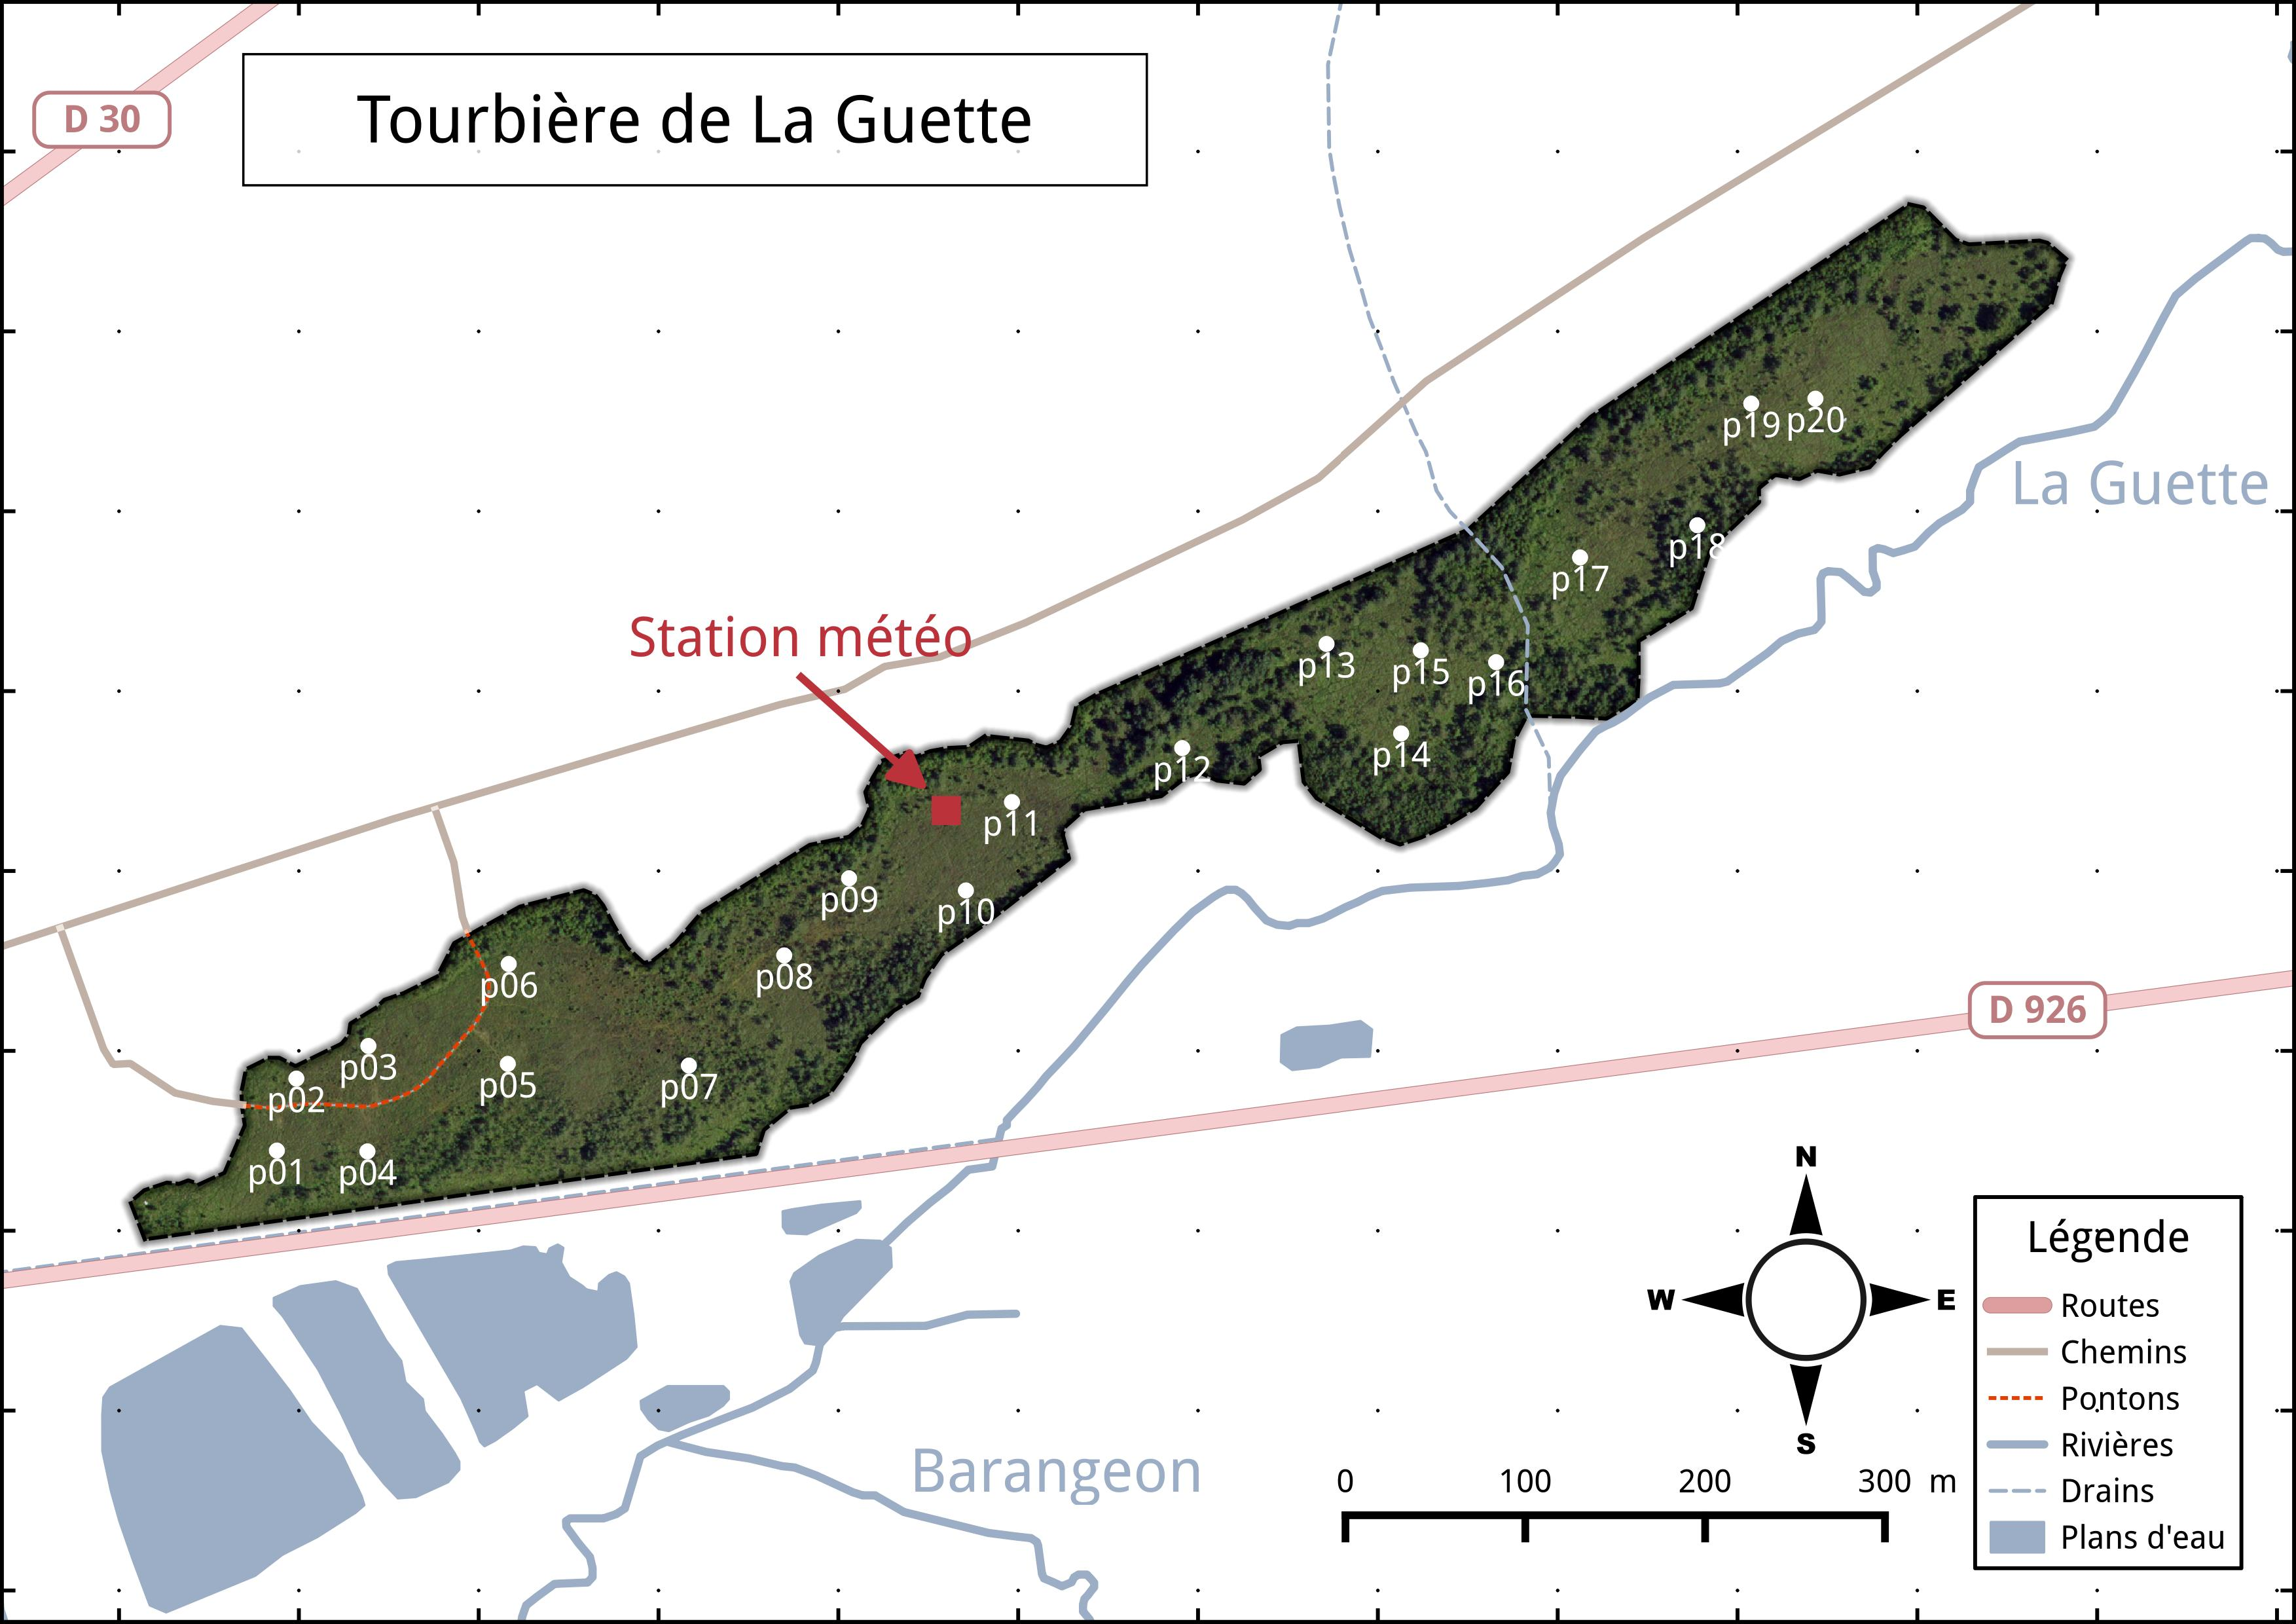
\includegraphics[width=\textwidth]{chap3/carteVS}
\caption{Répartition des 20 placettes de mesures suivant un échantillonnage aléatoire stratifié.}
\label{fig:carteVS}
\end{figure}


Les mesures des flux de \coo et de \chh ont été effectuées en utilisant la méthode décrite dans la partie~\ref{sec:clsd_chbr_method}.
En juin 2011, 20 placettes ont été installées\footnote{je remercie ici Sébastien Gogo pour avoir installé ces placettes sur le terrain avant même mon arrivée.} selon un échantillonnage aléatoire stratifié:
La surface de la tourbière a été divisée selon une grille de 20 mailles et un point choisi aléatoirement dans chaque maille localise chaque placette.
La taille de la maille a été ajustée de manière à avoir vingt 20 carrés sur la surface de la tourbière.
Cette méthode permet de conserver un échantillonnage aléatoire tout en étant assuré d'avoir une représentativité spatiale du site homogène. 
Les placettes, délimitées par des piquets, occupaient une surface de \SI{4}{\square\metre} (2$\times$\SI{2}{\metre}), à l'intérieur de laquelle ont été installé de façon permanente un piézomètre et une embase permettant la mesure des flux de gaz (Les embases sont décrites dans le chapitre~\ref{ch:ch2}, partie~\ref{subsec:ss_mes_co2}).
Usuellement les placettes sont séparées en groupes micro-topographiques (Figure~\ref{fig:microtopo}), avec des embases positionnées sur les buttes (\textit{hummock}), les trous (\textit{hollows}) et les zones d'eau libre (\textit{pool}) \citep{Alm1997,waddington2000}.
Ou encore selon différent traitements, réhabilité/non réhabilité, exploité/non exploité, manipulé/non manipulé \citep{bortoluzzi2006a,strack2013}.
Ceci a l'avantage de permettre une distinction fine des capacités sources/puits mais a l'inconvénient du placement proche des embases les unes des autres limitant la représentativité spatiale des mesures.
Elles peuvent également être séparées en zone dans la tourbière, haut-marais \textit{versus} bas-marais, ou réhabilité \textit{versus} non-réhabilité.
Afin de gagner en représentativité spatiale, la taille du site le permettant, il a donc été décidé de positionner des placettes sur l'ensemble du site.
%De plus, du fait de l'omniprésence de végétation vasculaire, et de la taille des chambres par rapport à la micro-topographie une telle approche était difficile à mettre en oeuvre.

Les flux de \coo et de \chh sont mesurés.
Des tests effectués sur la tourbière ayant montré des émissions nulles de N$_{2}$O, ce gaz n'a pas été étudié.
Les mesures de \coo ont été effectuées de mars 2013 à février 2015, avec une fréquence quasiment mensuelle (20 campagnes, pour 24 mois de mesures). Les mesures de \chh ont été effectuées avec une fréquence et sur un nombre d'embases inférieur (12 campagnes, 5 embases).
Ceci a été déterminé par la difficulté de déploiement \textit{in-situ} de l'instrument SPIRIT.
Il est lourd, difficilement transportable dans un milieu tourbeux et nécessite entre chaque déplacement un temps de mise en marche/arrêt important : plus de \SI{30}{\minute}.
% (lourd, difficilement transportable dans un milieu tourbeux).

Les facteurs contrôlant mesurés manuellement sont la pression atmosphérique, le rayonnement photosynthétique actif (\textit{photosyntheticaly active radiation}, PAR), les températures du sol à différentes profondeurs, la végétation (pourcentage de recouvrement), le niveau de la nappe d'eau.
Des prélèvements d'eau ont été effectués chaque mois pour mesurer le pH et la conductivité (mesures effectuées sur le terrain après les mesures de flux).
Les échantillons ont été congelés pour la mesure ultérieure de la concentration en carbone organique dissout.
Les mesures de recouvrement de la végétation ont été sommées par strate végétale.
On utilisera donc RSM, RSA, RSH pour distinguer les recouvrements respectif de la strate muscinale (\textit{Sphagnum spp.}), arbustive (\textit{Erica tetralix} et \textit{Calluna vulgaris}), et herbacée (\textit{Molinia caerula} et \textit{Eriophorum augustifolium}).
Un indice de végétation, représentant la quantité de végétation présente dans une embase est également calculé de la façon suivante : 

\begin{equation}
IV = \frac{RSM + RSA + RSH}{\sum R{max}}
\end{equation}

Avec :
\begin{itemize}
\item $\sum R_{max}$ La somme des recouvrements maximum par strates.
\end{itemize}

L'ensemble de ces mesures nécessitant d'accéder aux placettes régulièrement, des planches de bois ont été utilisées comme pontons mobiles pour limiter les perturbations. La dispersion des placettes sur l'ensemble du site a rendu impossible une installation plus permanente.

Les mesures automatiquement acquise via une station météo Campbell\textsuperscript{\textregistered} sont la température de l'air, température de la tourbe à \num{-5}, \num{-10}, \num{-20} et \SI{-40}{\centi\metre} de profondeur, vitesse et direction du vent, humidité relative de l'air, rayonnement solaire, pression atmosphérique.

\subsection{Modélisation du bilan de C}

\subsubsection{Estimation du bilan et variabilité temporelle}

Pour estimer le bilan de carbone du site il est nécessaire d'établir des modèles reliant des flux mesurés ponctuellement avec des variables explicatives mesurées à haute fréquence (e.g. relation entre la respiration de l'écosystème et la température de l'air).
Ces relations empiriques permettront d'interpoler les données acquises mensuellement sur l'ensemble des deux années de mesure et de reconstituer ainsi une chronique de flux dont l'intégration dans le temps permettra d'estimer une quantité sur l'année.
Pour établir ces modèles empiriques les données acquises ont été moyennées par campagne de mesure.
Ceci permettant, dans un premier temps, de s'affranchir de la variabilité spatiale des flux pour se concentrer sur la variabilité temporelle.
Les relations entre flux et facteurs contrôlant ont ensuite été étudiées deux à deux.

La RE, et l'ENE sont mesurés directement sur le terrain.
Cependant afin d'établir le bilan de C tout en gardant une discrimination entre flux d'entré et de sortie la RE et la PPB (obtenue grâce à l'équation PPB = ENE - RE) ont été modélisé séparément.
%Les flux de \coo ont été modélisé en partant de l'équation ENE = PPB - RE, et le bilan a été établi en estimant de façon séparée la PPB et la RE.
%Cette séparation permettant de distinguer si une variation du bilan est liée à l'un ou l'autre des flux ou bien aux deux.
Les flux en phase gazeuse ont été modélisés en partant d'équations usuellement utilisées et dans lesquelles la température est le facteur contrôlant majeur.
Puis les résidus\footnote{Valeurs moyennes - Valeurs moyennes estimées} de ces modèles de base ont ensuite été étudiés en fonction des facteurs de contrôle restant.
Dans le cas où une tendance est visible, le facteur est intégré.

Les modèles ont été comparés avec différents indicateurs : Le coefficient de détermination (R\textsuperscript{2}), l'erreur standard normalisée (\textit{Normalised Root Mean Square Error}, NRMSE) et le critère d'information d'Akaike (\textit{Akaike Information Criterion}, AIC).
Le R$^{2}$ est utilisé comme indicateur de la proportion de la variabilité des données expliquée par le modèle, sa valeur est comprise entre 0 et 1.
La RMSE et sa normalisation par la moyenne NRMSE sont utilisés comme indicateur de l'écart entre les données mesurées et les données modélisées.
L'AIC permet de déterminer la pertinence de l'ajout d'un paramètre sur la représentation des données par le modèle.

La température a été choisie comme base de départ à la construction des modèles de RE et PPBsat, à la fois car c'est le facteur de contrôle le plus souvent invoqué et à la fois car les corrélations avec les flux étaient les plus forte.
Concernant la respiration de l'écosystème, les températures utilisées dans la littérature sont variables.
La température la plus utilisée est la température du sol à \SI{-5}{\centi\metre}  \citep{ballantyne2014}.
La température de l'air et la température du sol à \SI{-10}{\centi\metre} sont aussi régulièrement utilisées \citep{bortoluzzi2006a,kim1992}.
Cette profondeur, \SI{-5}{\cm}, est régulièrement utilisée car c'est dans la tourbe, proche de la surface que la respiration du sol est la plus importante.
\plop %\textbf{production CO2 ? profils ?}
C'est également à des profondeurs relativement faibles que se situent la majorité des racines \plop.
La respiration liée aux racines (autotrophe et hétérotrophe stimulée par les exsudats racinaires) peut contribuer à la respiration de l'écosystème pour 35 à \SI{60}{\percent} \citep{silvola1996,crow2005}.
La RE est estimée directement à partir des données acquises moyennées en partant de la température connue pour contrôler une grande partie de ce flux.
Les modèles les plus fréquemment utilisés (linéaire, exponentiel, arrhénius) ont été testés.

Pas de consensus émerge de la littérature quant aux facteurs contrôlant les émissions de \chh.
La température, \citep{alm1999,bubier1995b}, le niveau de la nappe \citep{bubier1993} et/ou la végétation \citep{bortoluzzi2006a} peuvent être utilisés isolement ou conjointement.

Après la phase de calibration, les facteurs de contrôle utilisés dans les modèles ont été évalués à l'aide de données indépendantes issues d'une autre expérimentation réalisée sur le même site en 2014.
%Cette dernière est également un suivi des mêmes flux de gaz, sur le même site pendant l'année 2014.
Les méthodes de mesures des flux sont strictement identiques à celles utilisées pour établir le bilan de carbone.
En revanche le positionnement des placettes est beaucoup plus classique : proches les unes des autres, et avec différents traitements.
Afin de pouvoir les comparer, seule les placettes de contrôles, (n'ayant donc subie aucune manipulation) de cette expérimentation seront utilisées soit 4 placettes dans une station en amont et 4 en aval de la tourbière de La Guette (plus de détails dans l'annexe~\ref{sec:carbiodiv}).
Le terme d'évaluation est préféré à celui de validation car le nouveau jeu de données utilisé, bien qu'indépendant de celui utilisé pour la calibration, n'a pas été acquis de manière strictement identique, notamment au niveau de la répartition des embases sur le site.

Enfin les facteurs contrôlants ont été interpolés au pas de mesure de la station météo présente sur le site, c'est-à-dire à l'heure.
Pour des données dont l'acquisition est manuelle uniquement, comme la végétation, une interpolation linéaire est faite entre les points de mesures.
Pour les données acquises à la fois automatiquement par la station météorologique et manuellement, comme la température de l'air ou de la tourbe, l'interpolation est faite à partir de la relation entre les mesures continues et ponctuelles.
Les flux sont ensuite recalculés (en \si{\micro\mole\per\square\meter\per\hour}) à l'échelle horaire sur les deux années de mesure puis sommés afin d'estimer les bilans de carbone.
Ces bilans sont par la suite exprimés en \si{\gram C m^{-2}} par période de temps (souvent l'année).

%L'interpolation étant soit une simple interpolation linéaire entre les données mensuelles, soit une relation avec les facteurs acquis par la station météorologique.
%À l'aide de ces interpolations et des équations les flux ont ensuite été recalculés, à l'échelle horaire, sur les 2 années de mesure puis les flux ont été sommés afin de calculer les bilans.
\begin{figure}
\centering
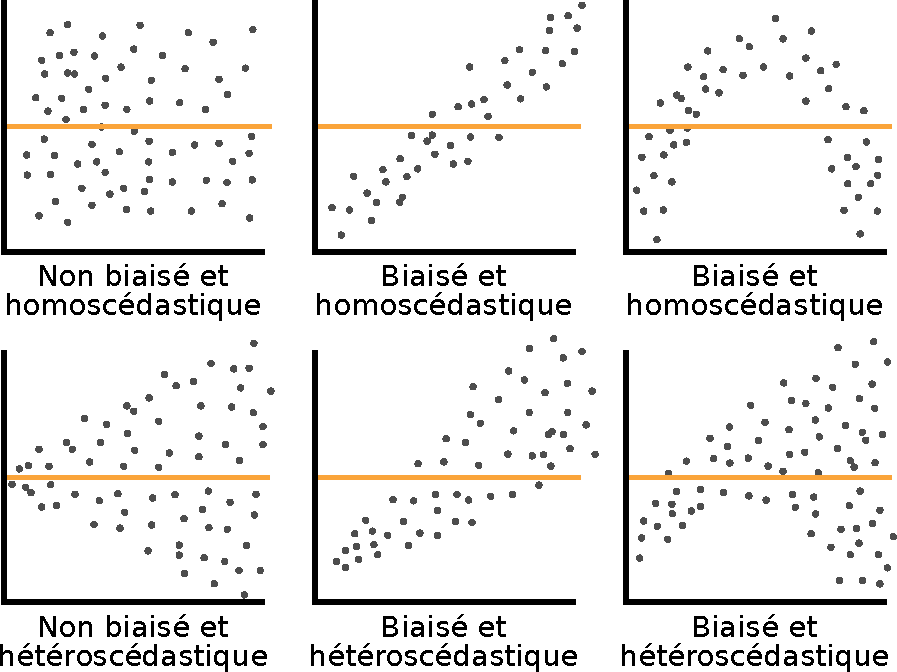
\includegraphics[width=\textwidth]{chap3/ref_resid}
\caption{Cas idéaux de distribution des résidus (source ?)}
\label{fig:ref_resid}
\end{figure}


\subsubsection{Étude de la variabilité spatiale}

Deux approches ont été testées afin de caractériser la variabilité spatiale des flux et du bilan.
La première consiste à calibrer par placette les modèles sélectionnés lors de la modélisation à l'échelle de l'écosystème.
Cette opération permet ainsi calculer des flux par placette et éventuellement un bilan.
L'inconvénient de cette méthode étant le faible nombre de points permettant la calibration des modèles conduisant éventuellement à une forte erreur sur l'estimation des paramètres voire à la non convergence des modèles.
La seconde approche permet de palier en partie à ce souci en calibrant les modèles à partir de groupes de placettes.
Ces ensembles de placette ont été fait en regroupant les placettes ayant la composition végétale la plus proche.
Ce choix se justifie par le fait que la végétation joue un rôle important tout en étant délicate à prendre en compte.
La température, plus facile à mesurer et le niveau de la nappe, qui n'a que peu varié, semblait des choix moins pertinent. 
Le partitionnement à été faite via une classification hiérarchique ascendante.
C'est une méthode déterministe qui consiste, à partir de l'ensemble des individus (ici nos différentes placettes de mesure), de les regrouper en classes de plus en plus grande.
Les points sont regroupés par similarité, les deux points les plus proches sont fusionnés, puis les deux suivants et ce jusqu'à ce qu'il ne reste qu'une seule classe.
Cette classification est généralement représentée par un dendrogramme, elle a été appliquée sur les recouvrements végétaux mesurés et permet de distinguer quatre groupes (Figure~\ref{fig:tree}).

\begin{figure}[t]
\centering
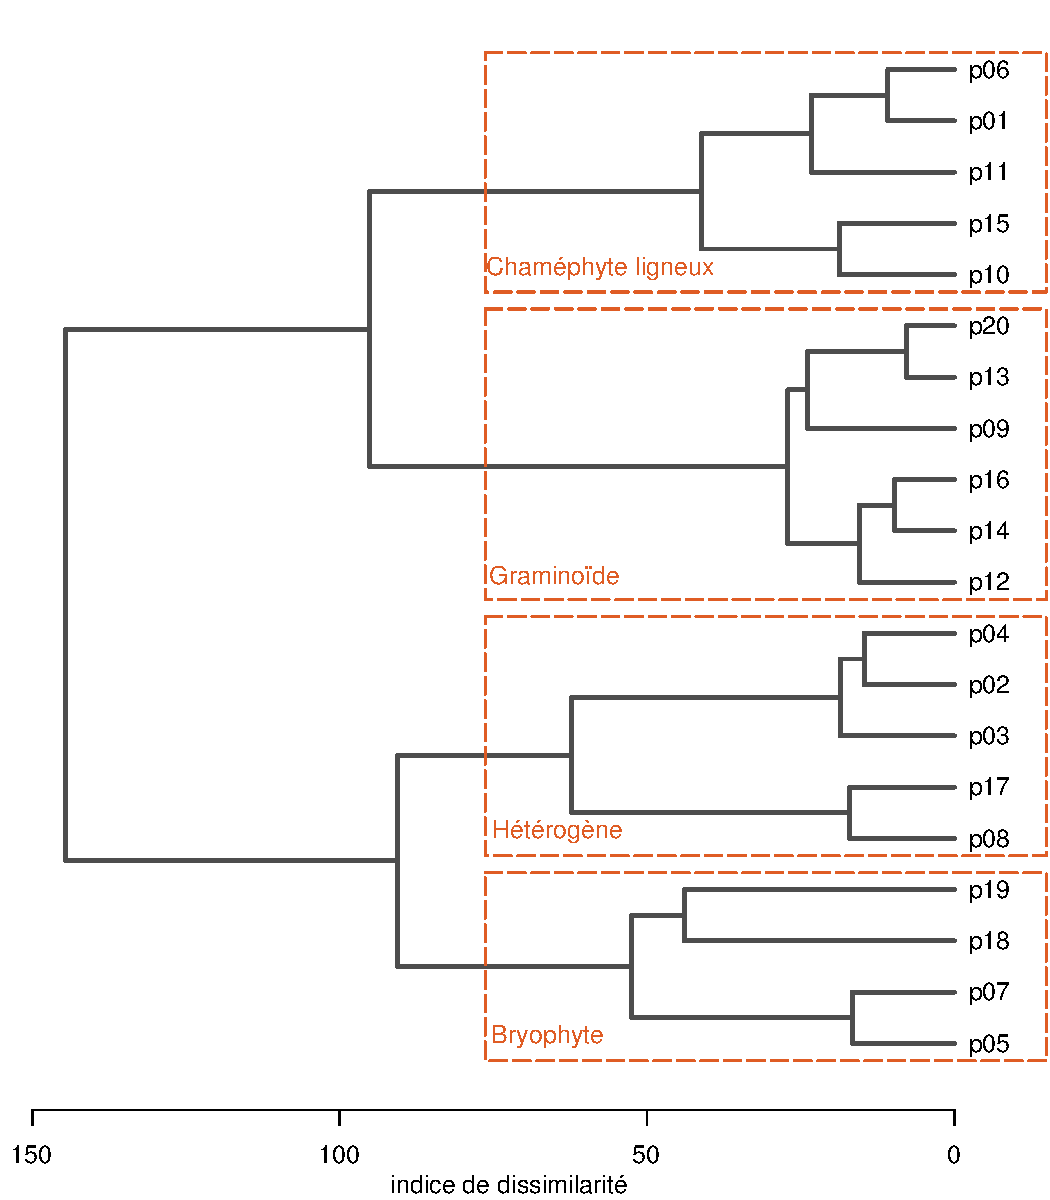
\includegraphics[width=\textwidth]{chap3/tree}
\caption{Partitionnement des placettes en fonction de leur similarité en termes de composition végétale (pourcentage des strates muscinales, herbacées et arbustives)}
\label{fig:tree}
\end{figure}



\section{Résultats}

\subsection{Cinétique des facteurs contrôlant et des flux sur la tourbière de La Guette}

\subsubsection{Les Facteurs contrôlant}

\begin{figure}
\centering
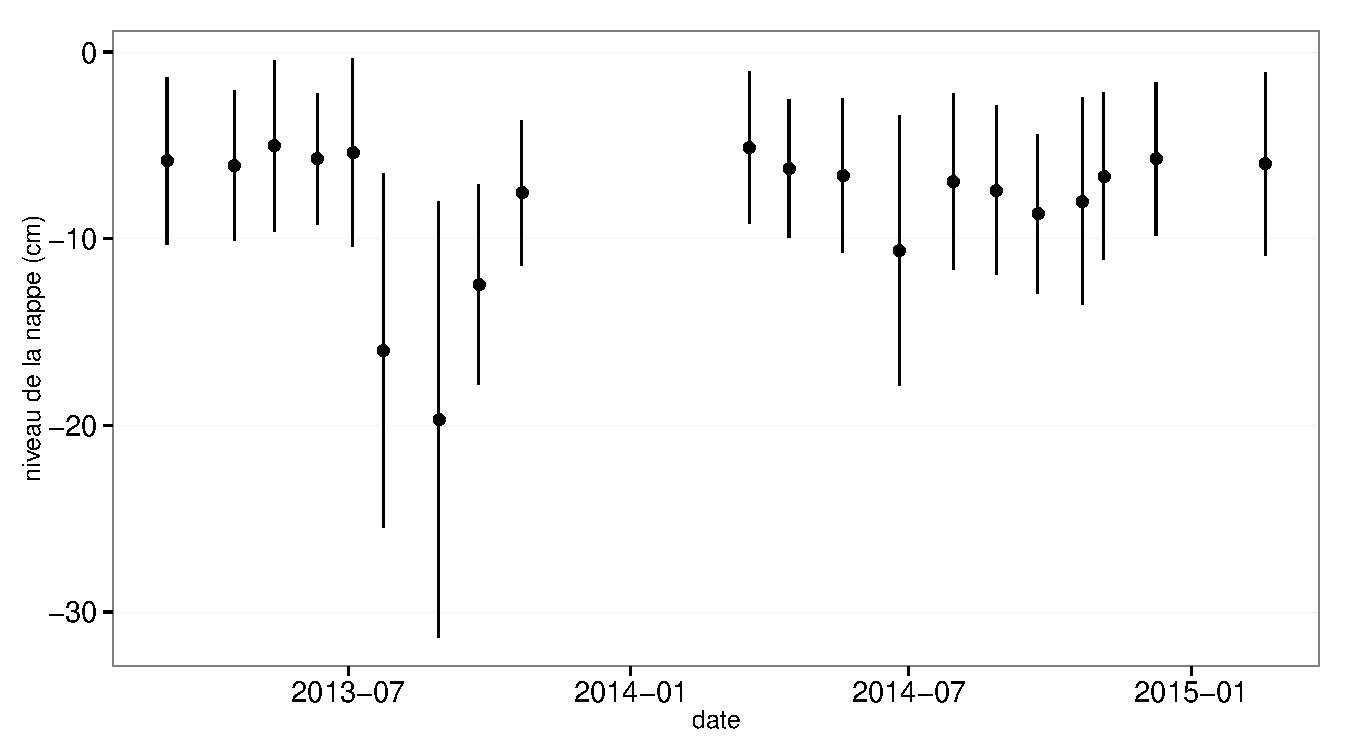
\includegraphics[width=\textwidth]{chap3/WTL_mean_evolution}
\caption{Évolution du niveau de la nappe moyen des 20 embases mesuré pendant la période de mesure (mars 2013 -- février 2015)}
\label{fig:WTL_mean_evolution}
\end{figure}

L'évolution du niveau de la nappe des 20 placettes est marquée par un étiage d'une vingtaine de centimètres en moyenne en 2013 et l'absence d'un étiage net en 2014 (Figure~\ref{fig:WTL_mean_evolution}).
Le niveau de la nappe moyen ne descend pas sous la barre des \SI{-10}{\cm} avec \num{-9.2(76)} et \SI{-7.1(48)}{\centi\metre} respectivement pour 2013 et 2014.
% ne descendant que rarement sous la barre des \SI{-10}{\cm}.
Ces observations sont cohérentes avec les mesures haute fréquence (Figure~\ref{fig:WTL}), et confirment l'étiage particulièrement haut de ces 2 années vis-à-vis des précédentes.

\begin{figure}
\centering
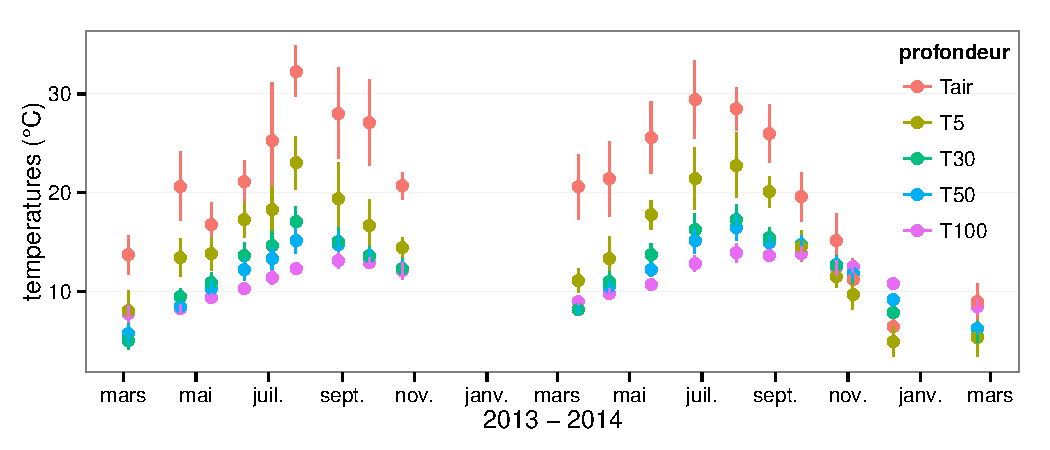
\includegraphics[width=\textwidth]{chap3/T_mean_evolution}
\caption{Évolution des températures de l'air (Tair) et du sol à \SIlist{-5;-30;-50;-100}{\centi\metre} (T5, T30, T50 et T100 respectivement) moyenne mesurée lors des campagnes de terrain de mars 2013 à février 2015}
\label{fig:T_mean_evolution}
\end{figure}

La température de l'air mesurée manuellement montre une variabilité saisonnière cohérente avec celle mesurées par la station météo. 
%bien que les valeurs semblent systématiquement supérieures.
La variabilité saisonnière de la température est également visible dans le sol avec cependant un amortissement et une diminution de la variabilité avec la profondeur (figure~\ref{fig:T_mean_evolution})
%chiffres ?

\begin{figure}
\centering
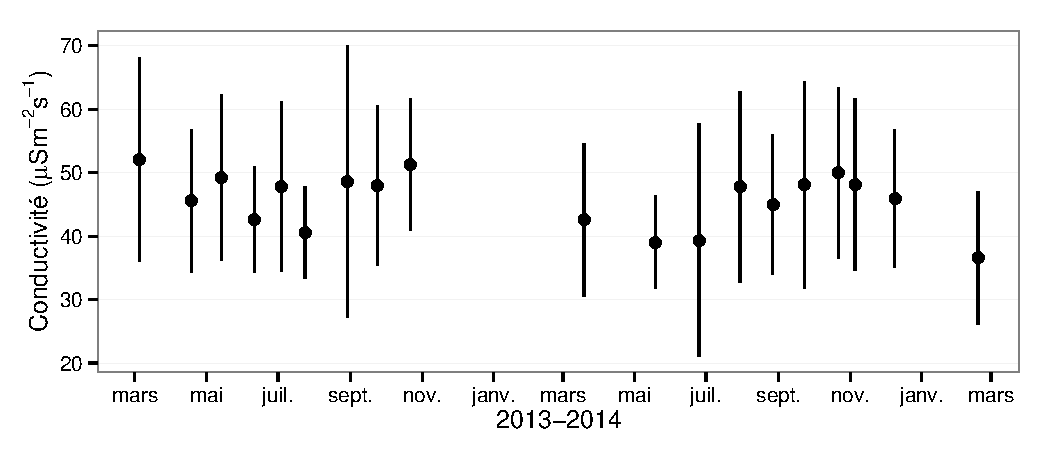
\includegraphics[width=\textwidth]{chap3/cond_mean_evolution}
\caption{Évolution de la conductivité pendant la période de mesure (mars 2013 -- février 2015)}
\label{fig:cond_mean_evolution}
\end{figure}

La conductivité moyenne mesurée sur le site varie entre \SIlist{35;55}{\usml} (figure~\ref{fig:cond_mean_evolution}).


\begin{figure}
\centering
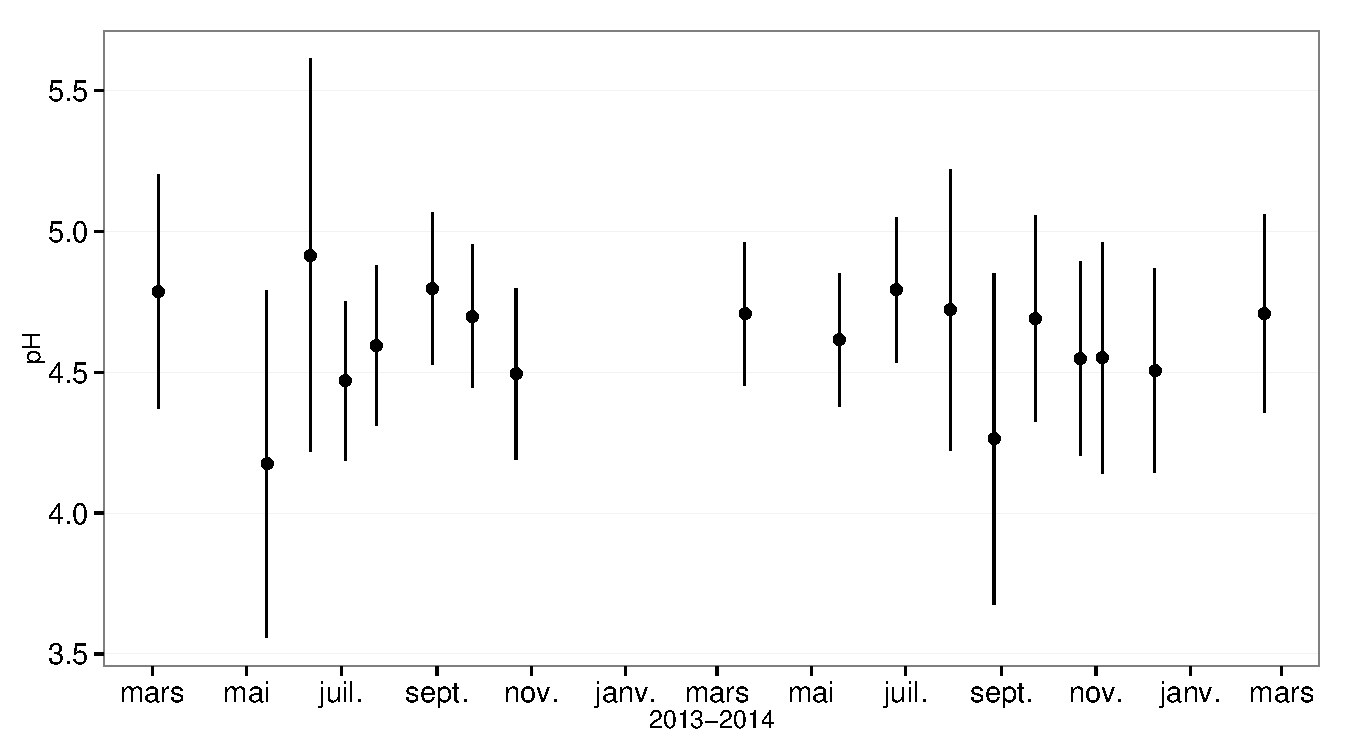
\includegraphics[width=\textwidth]{chap3/pH_mean_evolution}
\caption{Évolution du pH pendant la période de mesure (mars 2013 -- février 2015)}
\label{fig:pH_mean_evolution}
\end{figure}


En moyenne le pH mesuré sur la tourbière de La Guette est compris entre 4 et 5 (figure~\ref{fig:pH_mean_evolution}).
Ces valeurs sont cohérentes avec la classification en \textit{poor-fen} du site .


%\begin{figure}
%\centering
%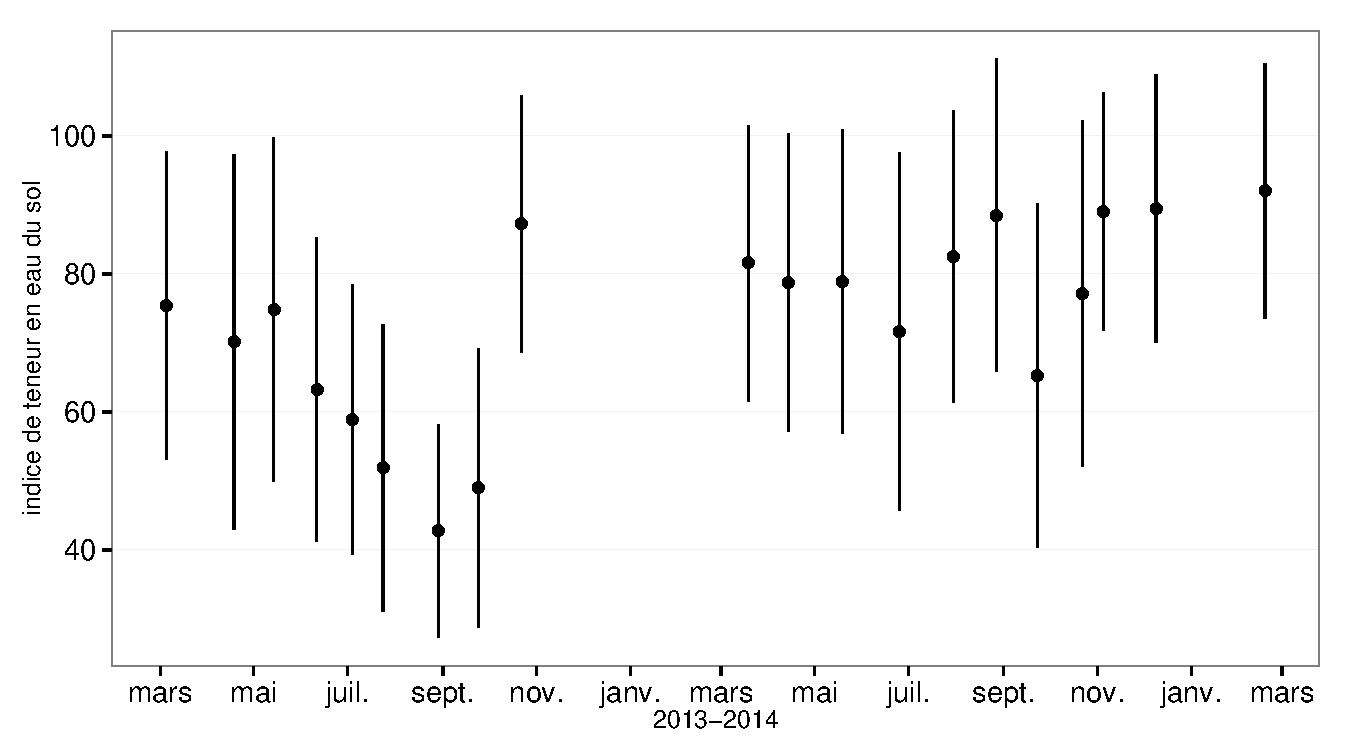
\includegraphics[width=\textwidth]{chap3/RH_mean_evolution}
%\caption{Évolution de la teneur en eau du sol pendant la période de mesure (mars 2013 -- février 2015)}
%\label{fig:RH_mean_evolution}
%\end{figure}

\begin{figure}
\centering
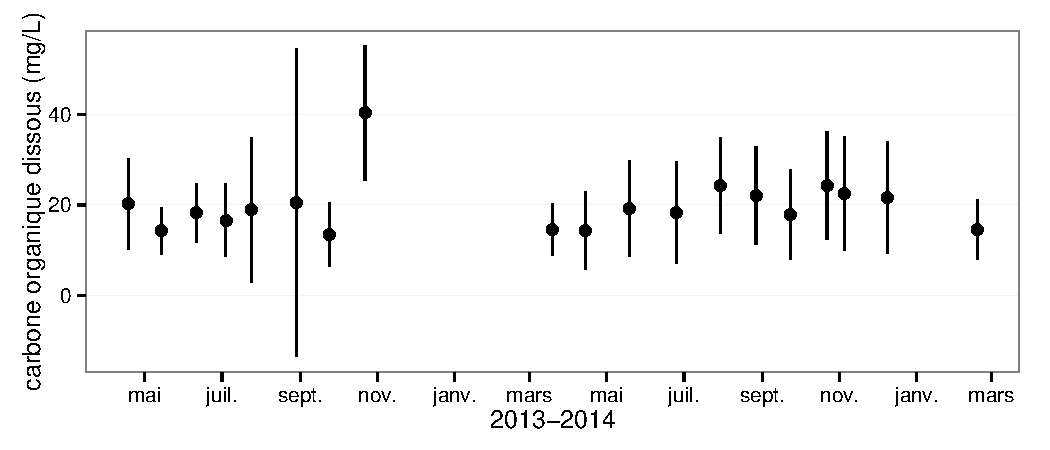
\includegraphics[width=\textwidth]{chap3/NPOC_mean_evolution}
\caption{Évolution de la concentration en carbone organique dissous dans l'eau du sol pendant la période de mesure (mars 2013 -- février 2015)}
\label{fig:NPOC_mean_evolution}
\end{figure}

La concentration en carbone organique dissout présente dans l'eau de la tourbière est compris en moyenne entre \num{10} et \SI{30}{\milli\gram\per\liter} (figure~\ref{fig:NPOC_mean_evolution}).

%\subsection{Évolution générale des flux de C sur la tourbière de La Guette}

\subsubsection{Les flux de carbone}

\begin{figure}
	\centering
	\begin{subfigure}[t]{\textwidth}
		\centering
		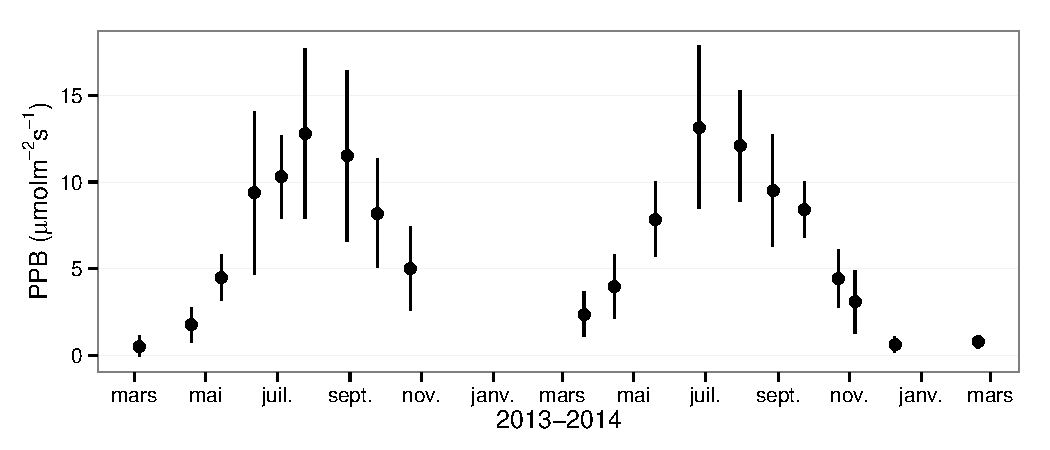
\includegraphics[width=\textwidth]{chap3/GPP_evolution_avg}
		\caption{Production primaire brute}
		\label{fig:GPP_evolution_avg}
	\end{subfigure}%
	
	\begin{subfigure}[t]{\textwidth}
		\centering
		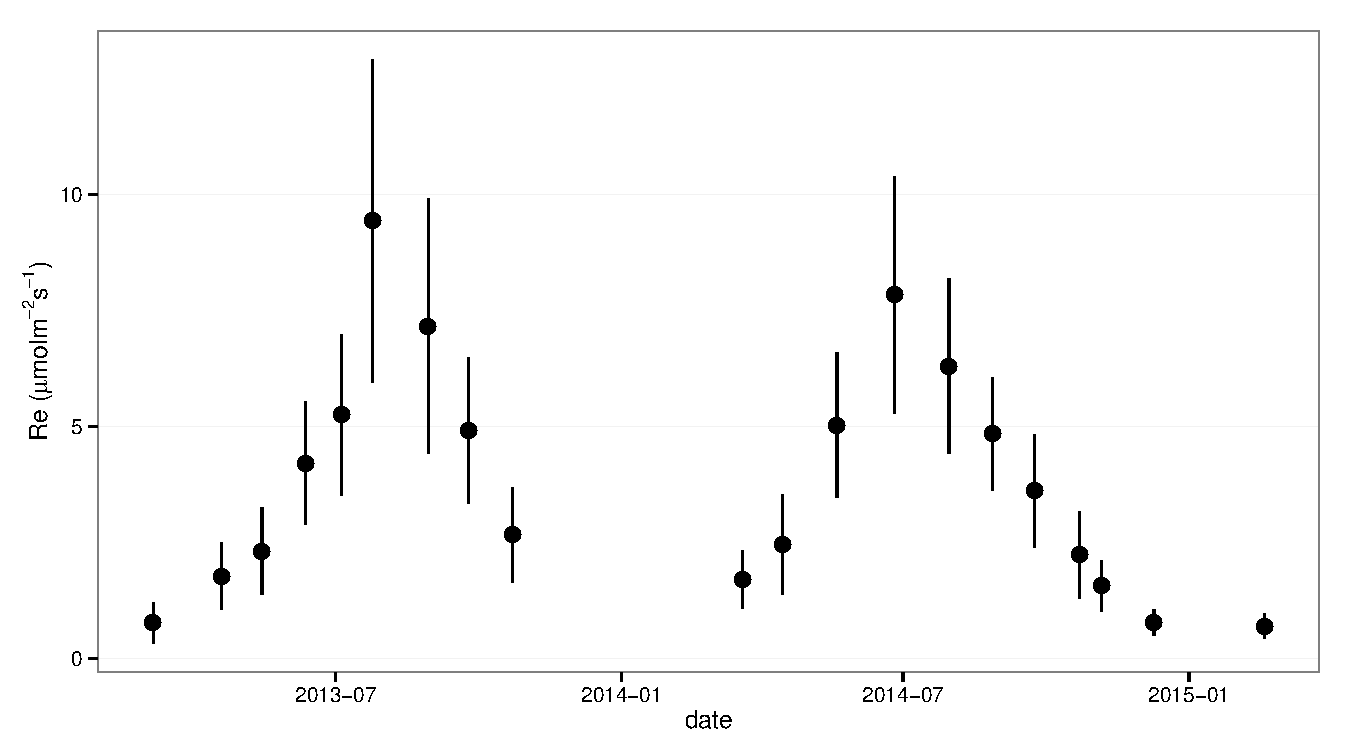
\includegraphics[width=\textwidth]{chap3/ER_evolution_avg}
		\caption{Respiration de l'écosystème}
		\label{fig:ER_evolution_avg}
	\end{subfigure}
	
	\begin{subfigure}[t]{\textwidth}
		\centering
		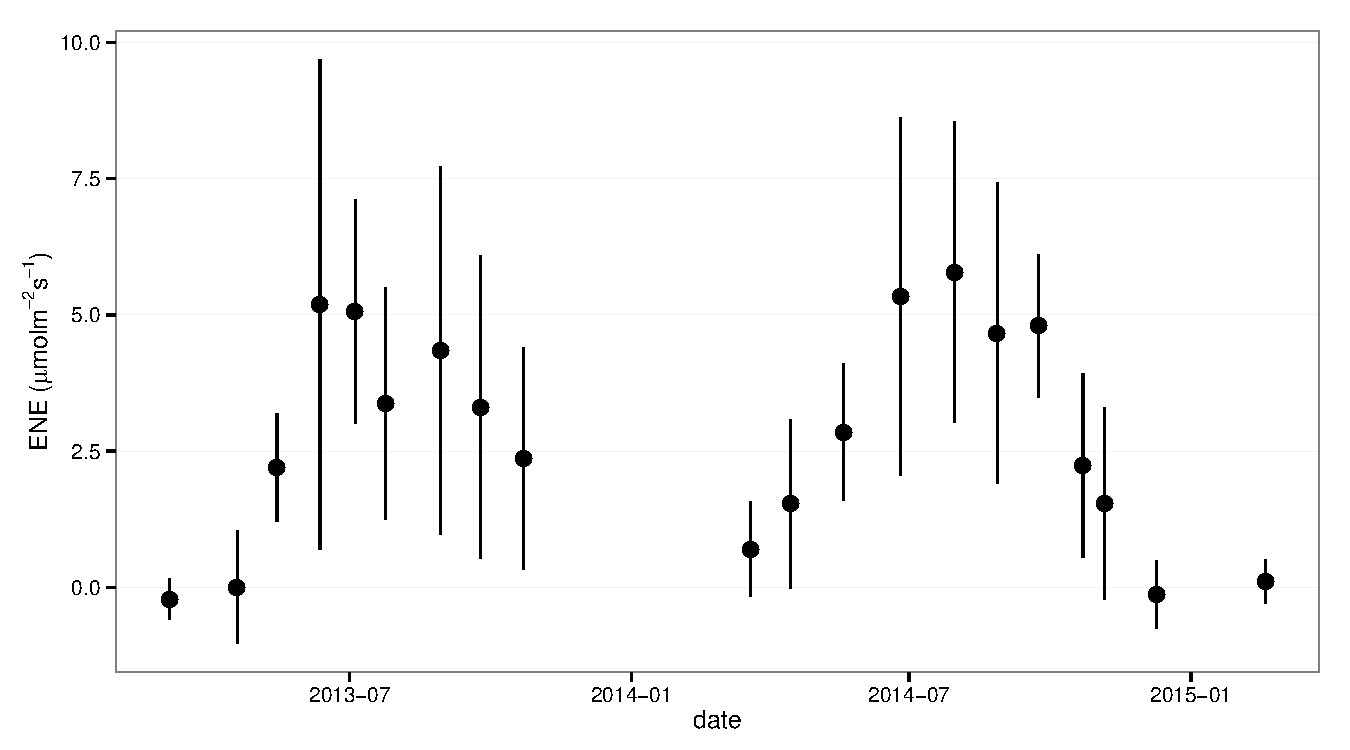
\includegraphics[width=\textwidth]{chap3/NEE_evolution_avg}
		\caption{Échange net de l'écosystème}
		\label{fig:NEE_evolution_avg}
	\end{subfigure}
\caption{Évolution du niveau de PPB, RE et ENE pendant la période de mesure. Moyenne des 20 embases de mars 2013 à février 2015.}
\label{fig:flux_evolution_avg}
\end{figure}

%\subsubsection{PBB}
L'ensemble des mesures de \coo s'étendent de mars 2013 à février 2015.
Cependant de novembre 2013 à février 2014 les mesures ont été interrompue suite à des problèmes techniques.
Les deux saisons de végétation, ont pu être mesurées dans leur ensemble, permettant d'avoir un jeu de données représentatif sur le fonctionnement de l'écosystème.
À noter également que pour l'ensemble des flux, la déviation standard augmente avec les valeurs mesurées.

En 2013, les valeurs de la PPB (flux de \coo entrant dans l'écosystème) augmentent au printemps et une partie de l'été avec un maximum de \SI{12.80(491)}{\uml} atteint fin juillet, avant de diminuer à partir d'août (Figure~\ref{fig:GPP_evolution_avg}).
En 2014 la PPB maximale est atteinte en juin (\SI{13.16(470)}{\uml}), soit environ un mois plus tôt que l'année précédente.
Puis pendant l'été et l'automne les valeurs décroissent jusqu'à être proche de 0.
En moyenne les valeurs de la PPB sont de \SI{7.12(519)}{\uml} en 2013 et de \SI{6.56(472)}{\uml} en 2014 (Figure~\ref{fig:GPP_evolution_avg}).

La RE (flux de \coo sortant de l'écosystème) en 2013 augmente pendant le printemps et une partie de l'été (Figure~\ref{fig:ER_evolution_avg}).
Elle atteint un maximum de \SI{9.43(348)}{\uml} en juillet avant de diminuer.
En 2014 la RE atteint, comme la PPB, son maximum plus tôt, en juin à \SI{7.83(255)}{\uml} avant de décroître jusqu'en hiver pour approcher des valeurs nulles.
La moyenne annuelle de RE en 2013 est de \SI{4.27(316)}{\uml}, ce qui est légèrement supérieure à celle de 2014 : \SI{3.63(256)}{\uml}(Figure~\ref{fig:ER_evolution_avg}).

Concernant l'ENE (bilan des flux de \coo entrant et sortant), elle augmente en 2013 jusque \SI{5.19(451)}{\uml}, avec un maximum en juin, avant de diminuer jusqu'à la fin de l'année.
Cependant, cette baisse est moins uniforme que celle des deux flux précédents, avec notamment une augmentation de l'ENE entre juillet et août 2013.
Ceci étant, il faut également noter les valeurs importantes de la déviation standard particulièrement en juin et en août.
En 2014, l'ENE maximum est atteinte en juillet avec \SI{5.79(277)}{\uml} avant qu'elle ne décroisse.
Cette baisse est cependant plus homogène qu'en 2013.
les moyennes de l'ENE en 2013 et 2014 sont très proche et sont respectivement de \SI{2.85(305)}{\uml} et \SI{2.93(277)}{\uml} (Figure~\ref{fig:NEE_evolution_avg}).

%\subsubsection{Le \chh}

Les flux de \chh comme ceux du \coo montre une variabilité saisonnière importante.
Cependant les flux de \chh mesurés sont un ordre de grandeur en dessous de ceux mesurés pour le \coo (Figure~\ref{fig:CH4_evolution_avg}).
À l'inverse de ce dernier, l'importance des flux de \chh mesurés en 2013 et 2014 est différente.
En 2013 les flux sont moins importants qu'en 2014 avec des maximum de \num{0.078} et \SI{0.196}{\uml} respectivement.

\begin{figure}
\centering
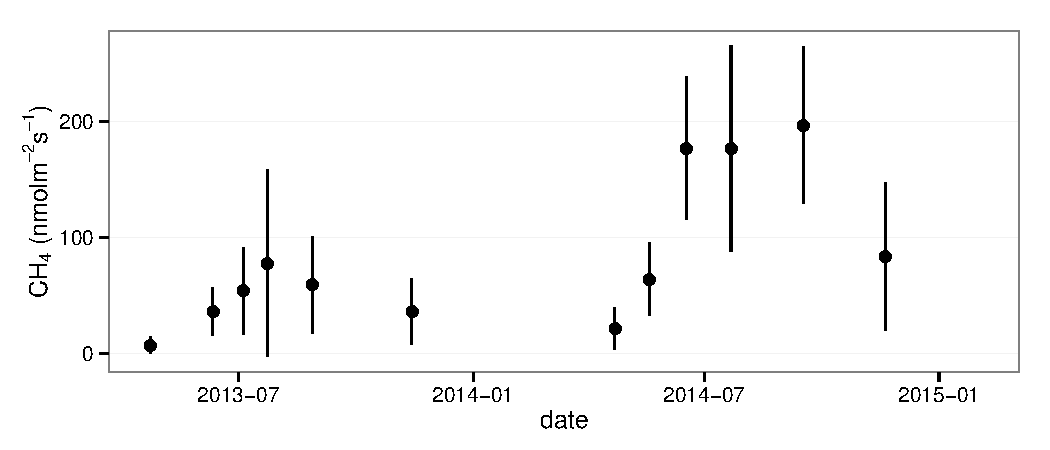
\includegraphics[width=\textwidth]{chap3/CH4_evolution_avg}
\caption{Évolution des flux de méthane moyen (N ?) pendant la période de mesure (mars 2013 -- février 2015)}
\label{fig:CH4_evolution_avg}
\end{figure}

%\subsubsection{Le Carbone Organique Dissous (COD)}
\begin{figure}
\centering
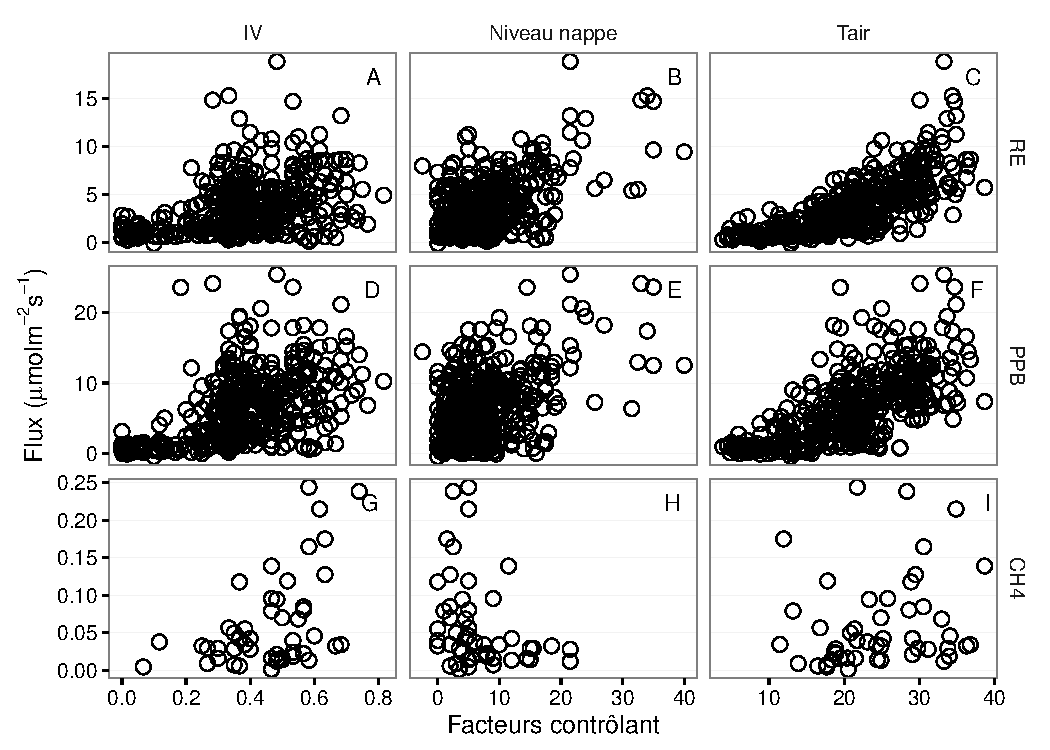
\includegraphics[width=\textwidth]{chap3/Fl_FC}
\caption{Relations entre les flux de gaz et une sélection de facteurs contrôlant}
\label{fig:Fl_FC}
\end{figure}

\subsubsection{Les relations flux gazeux et facteurs contrôlant}

Comme précisé précédemment, le niveau de la nappe n'a que peu varié pendant les deux années de mesures.
De ce fait aucune relation claire ne se distingue entre les flux et le niveau de la nappe que ce soit pour le \coo (PPB et RE) ou le \chh (Figure~\ref{fig:Fl_FC}).
La PPB et la RE présentent cependant des relations avec la température de l'air, et l'indice de végétation, même si pour ce dernier les tendances sont moins claires, particulièrement pour la RE (Figure~\ref{fig:Fl_FC}).
Le \chh quant à lui ne présente pas de relation avec la température de l'air, mais une tendance exponentielle est visible vis-à-vis de l'indice de végétation (Figure~\ref{fig:Fl_FC}).
\textbf{(\chh et Température dans la tourbe ?)}

\subsection{Sélection des modèles}

\subsubsection{La Production Primaire Brute}

\begin{figure}
\centering
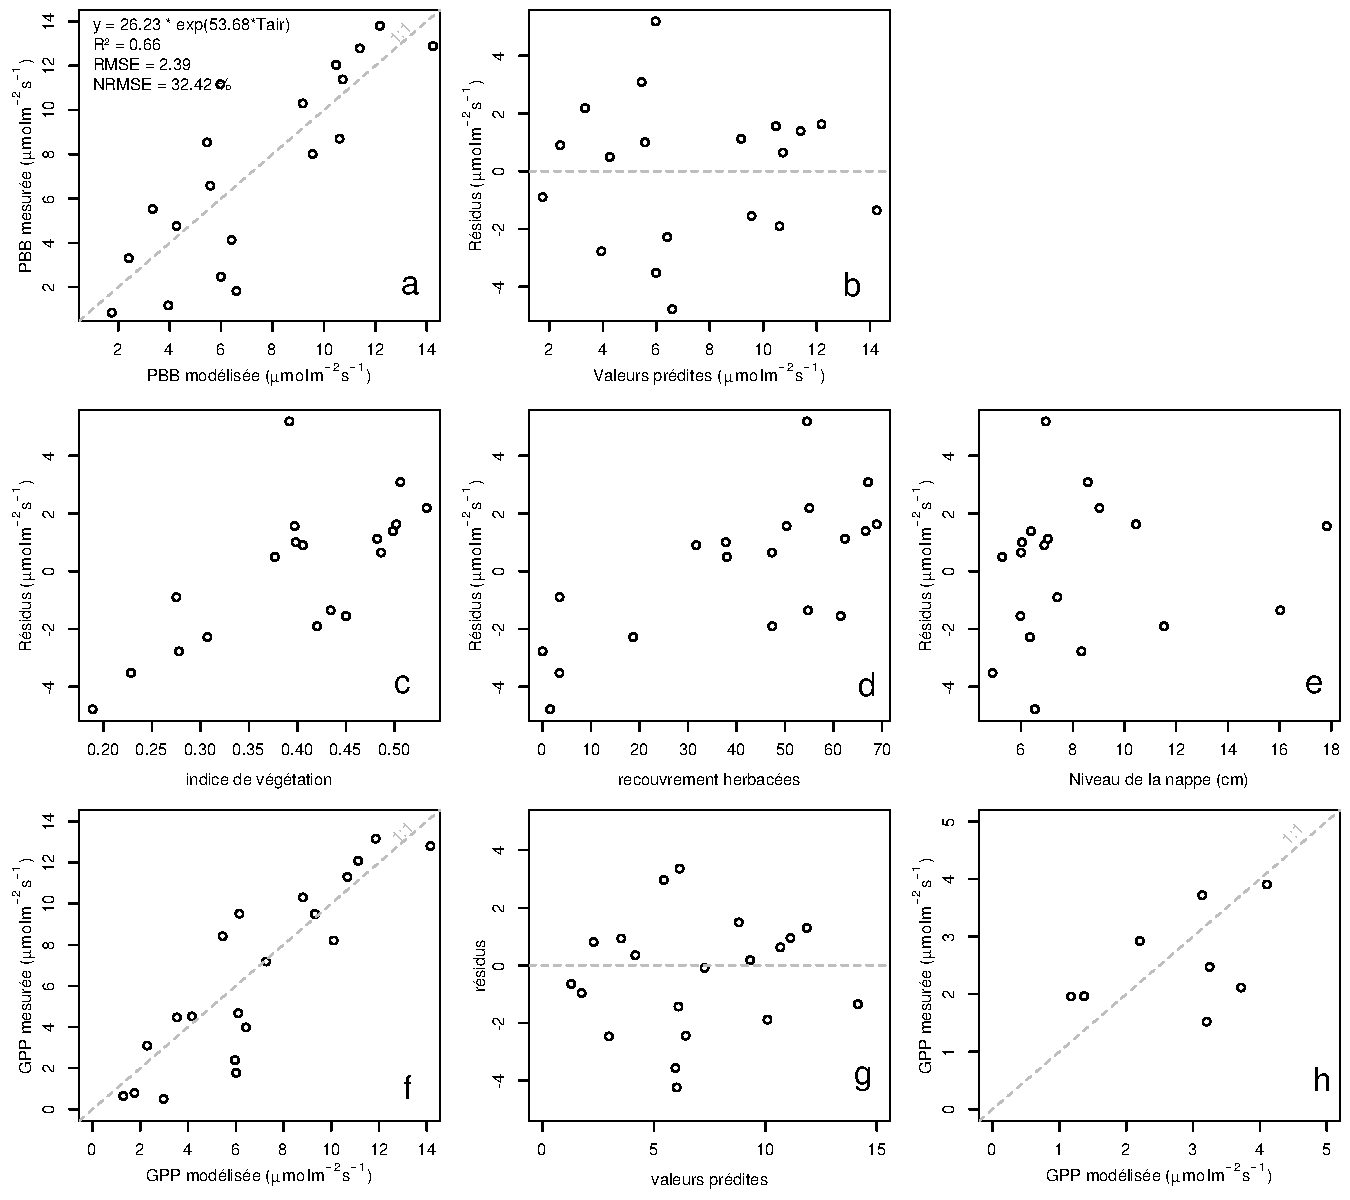
\includegraphics[width=1.15\textwidth, center]{chap3/mdl_GPP_Tair}
\caption{PPBsat modèles Tair utilisant l'équation~\ref{eq:juneTair}}
\label{fig:mdl_GPP_Tair}
\end{figure}

L'estimation de la PPB se fait en deux étapes.
Dans un premier temps on estime le potentiel maximum de photosynthèse à un instant donné dans des conditions de lumière saturante (PPBsat).
Ce potentiel peut varier avec les conditions environnementales et a été déterminé en utilisant l'équation de \citep{june2004} qui relie la vitesse de transport des électrons photosynthétiques à lumière saturante à la température :

\begin{equation}\label{eq:juneTair}
PPBsat = a * exp(\frac{Tair - b}{c})^2
\end{equation}

Avec :
\begin{itemize}
\item $a$ la vitesse de transport des électrons photosynthétique à lumière saturante
\item $b$ la température optimale pour ce transport
\item $c$ la différence de température à laquelle à laquelle PBBsat vaut e$^{-1}$ de sa valeur à la température optimale
\end{itemize}

À partir de ce potentiel à lumière saturante, la PPB est estimée en prenant en compte la luminosité.
On utilise l'équation~\ref{eq:PPB_bubier} proposée par \citep{bubier1998} et régulièrement et majoritairement utilisée \citep{bortoluzzi2006a,worrall2009}:

\begin{equation} \label{eq:PPB_bubier}
PPB = \frac{PPBsat * a * PAR}{PPBsat + a * PAR}
\end{equation}

L'utilisation de l'équation de June seule, avec la température de l'air comme variable explicative de la PPBsat, permet d'expliquer 66 \% des variations observées avec une erreur standard de l'estimation de \SI{32}{\percent} (Figure~\ref{fig:mdl_GPP_Tair}-a).
Les résidus de ce modèle se répartissent de façon relativement homogène et non biaisée (Figure~\ref{fig:mdl_GPP_Tair}-b).
Corrélés avec l'indice de végétation IV, ils présentent une tendance linéaire croissante (Figure~\ref{fig:mdl_GPP_Tair}-c).
On observe la même tendance avec le recouvrement de la strate herbacée avec une dispersion des points plus importante (Figure~\ref{fig:mdl_GPP_Tair}-d).
Par contre aucune tendance particulière n'est visible vis-à-vis du niveau de la nappe (Figure~\ref{fig:mdl_GPP_Tair}-e)
Le recouvrement des sphaignes (non présenté) ne montre également, aucune tendance avec les résidus de cette équation.
La PPB calculée à partir de l'équation~\ref{eq:juneTair} montre une erreur standard de \SI{31}{\percent}, du même ordre de grandeur que celle de PPBsat (Figure~\ref{fig:mdl_GPP_Tair}-f) et les résidus se répartissent de façon relativement homogène et non biaisée (Figure~\ref{fig:mdl_GPP_Tair}-g).
Cependant l'évaluation du modèle sur les données de tests montre une erreur standard de l'estimation plus forte qui atteint \SI{47}{\percent}(Figure~\ref{fig:mdl_GPP_Tair}-h).
Par ailleurs une forte incertitude est présente concernant l'estimation des paramètres qui ont tous une erreur standard importante, parfois plus importante que la valeur du paramètre, et une faible significativité (Tableau~\ref{table:mdl_par}).
Afin de prendre en compte la tendance linéaire entre les résidus et l'indice de végétation (IV) le modèle est adapté pour y intégré une fonction linéaire de la végétation :

\begin{equation}\label{eq:juneTairIV}
PPBsat = (a * IV + d) * exp(\frac{T - b}{c})^2
\end{equation}

\begin{figure}
\centering
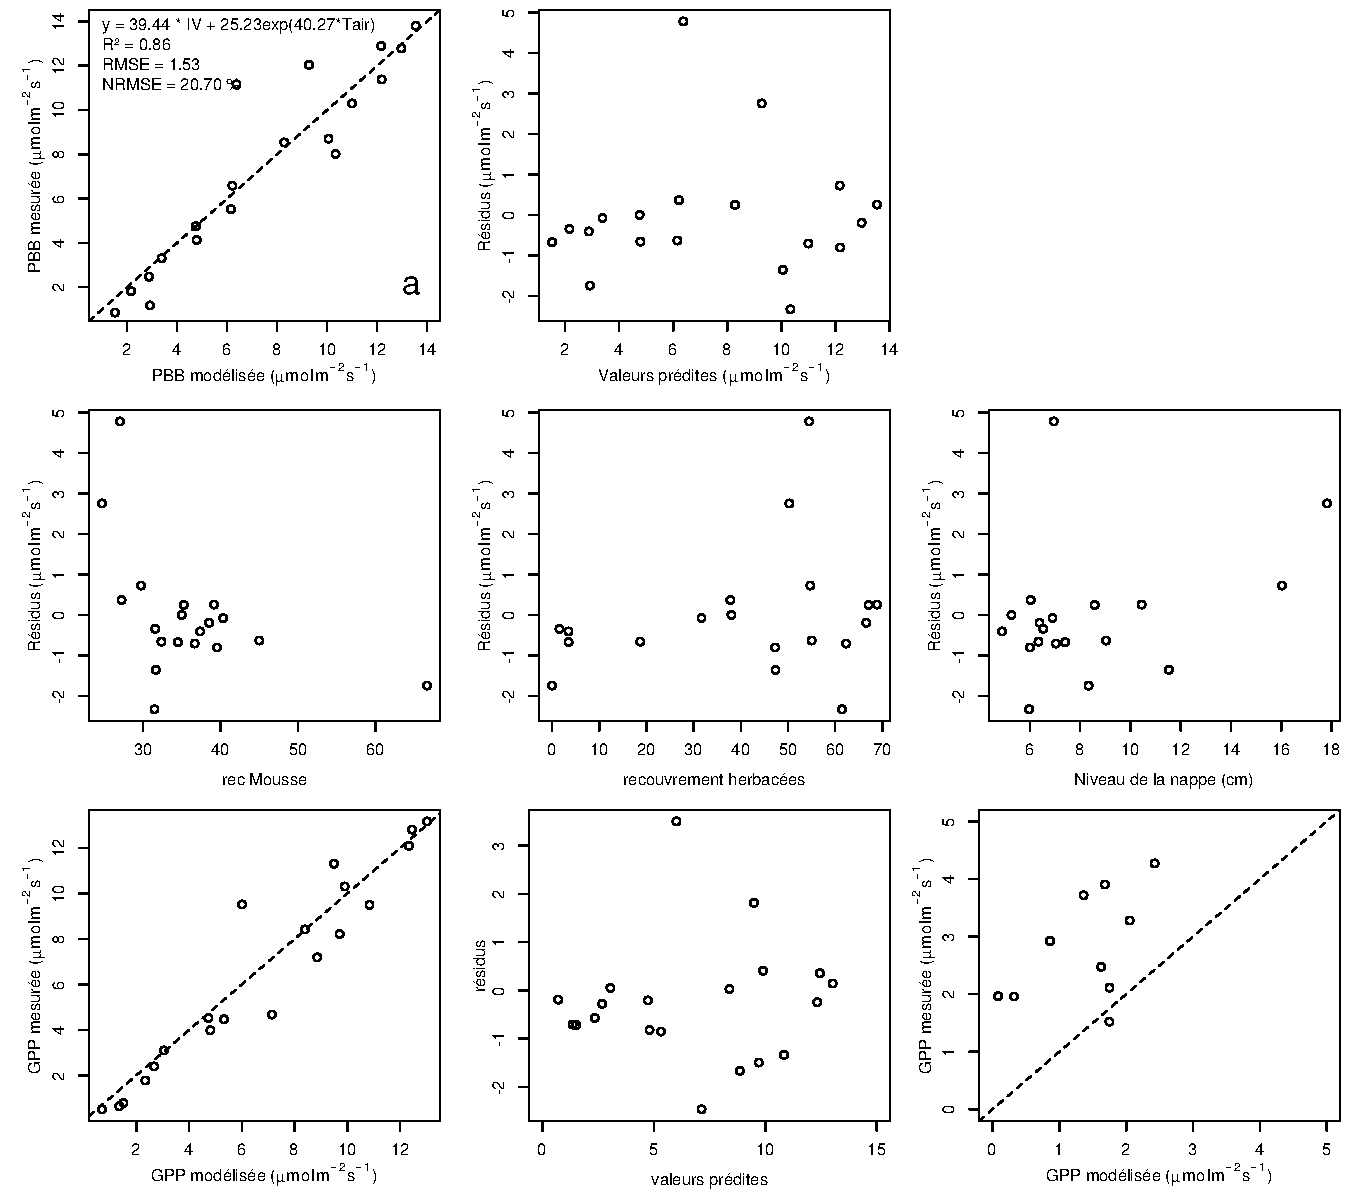
\includegraphics[width=1.15\textwidth, center]{chap3/mdl_GPP_TairIV}
\caption{PPBsat modèles Tair utilisant l'équation~\ref{eq:juneTairIV}}
\label{fig:mdl_GPP_TairIV}
\end{figure}

Cette nouvelle équation permet d'expliquer une part plus importante des variations de PPBsat (R$^{2}$ = 0,85) et augmente la proximité entre les données mesurées et les données modélisées : l'erreur standard diminue à \SI{21}{\percent}. (Figure~\ref{fig:mdl_GPP_TairIV}-a).
Les résidus de cette équation semblent répartis de façon moins homogène que précédemment.
On observe notamment un resserrement des points autour de zéro à l'exception d'un point de valeur supérieur à \num{4}.
Le biais reste malgré tout léger au regard de l'amélioration apportée.
Aucune tendance claire ne se dégage des résidus lorsqu'ils sont mis en relation avec des facteurs contrôlant tel que les recouvrements végétaux (sphaignes, herbacées), ou le niveau de la nappe (Figure~\ref{fig:mdl_GPP_TairIV}-c,d,e).
Comme précédemment, l'erreur standard de la PPB, de \SI{19}{\percent}, est du même ordre de grandeur que celle de PPBsat.
Pour PPBsat comme pour PPB l'erreur standard diminue avec l'ajout de l'indice de végétation lors de la calibration.
En revanche, l'évaluation sur les données de test de ce dernier modèle montre une erreur importante (\SI{58}{\percent}), supérieure à celle du modèle ne prenant pas en compte la végétation.
Cette évaluation montre également une tendance importante à sous-estimer les valeurs mesurées.
Néanmoins ce modèle intégrant la végétation permet de diminuer de façon importante l'erreur standard associée à l'estimation des paramètres de l'équation.
Dans la suite du texte le modèle permettant d'estimer la PPB à partir des équations~\ref{eq:juneTair} et \ref{eq:PPB_bubier} sera nommé PPB-1 et celui utilisant les équations~\ref{eq:juneTairIV} et \ref{eq:PPB_bubier} sera nommée PPB-2.


%\begin{figure}
%\centering
%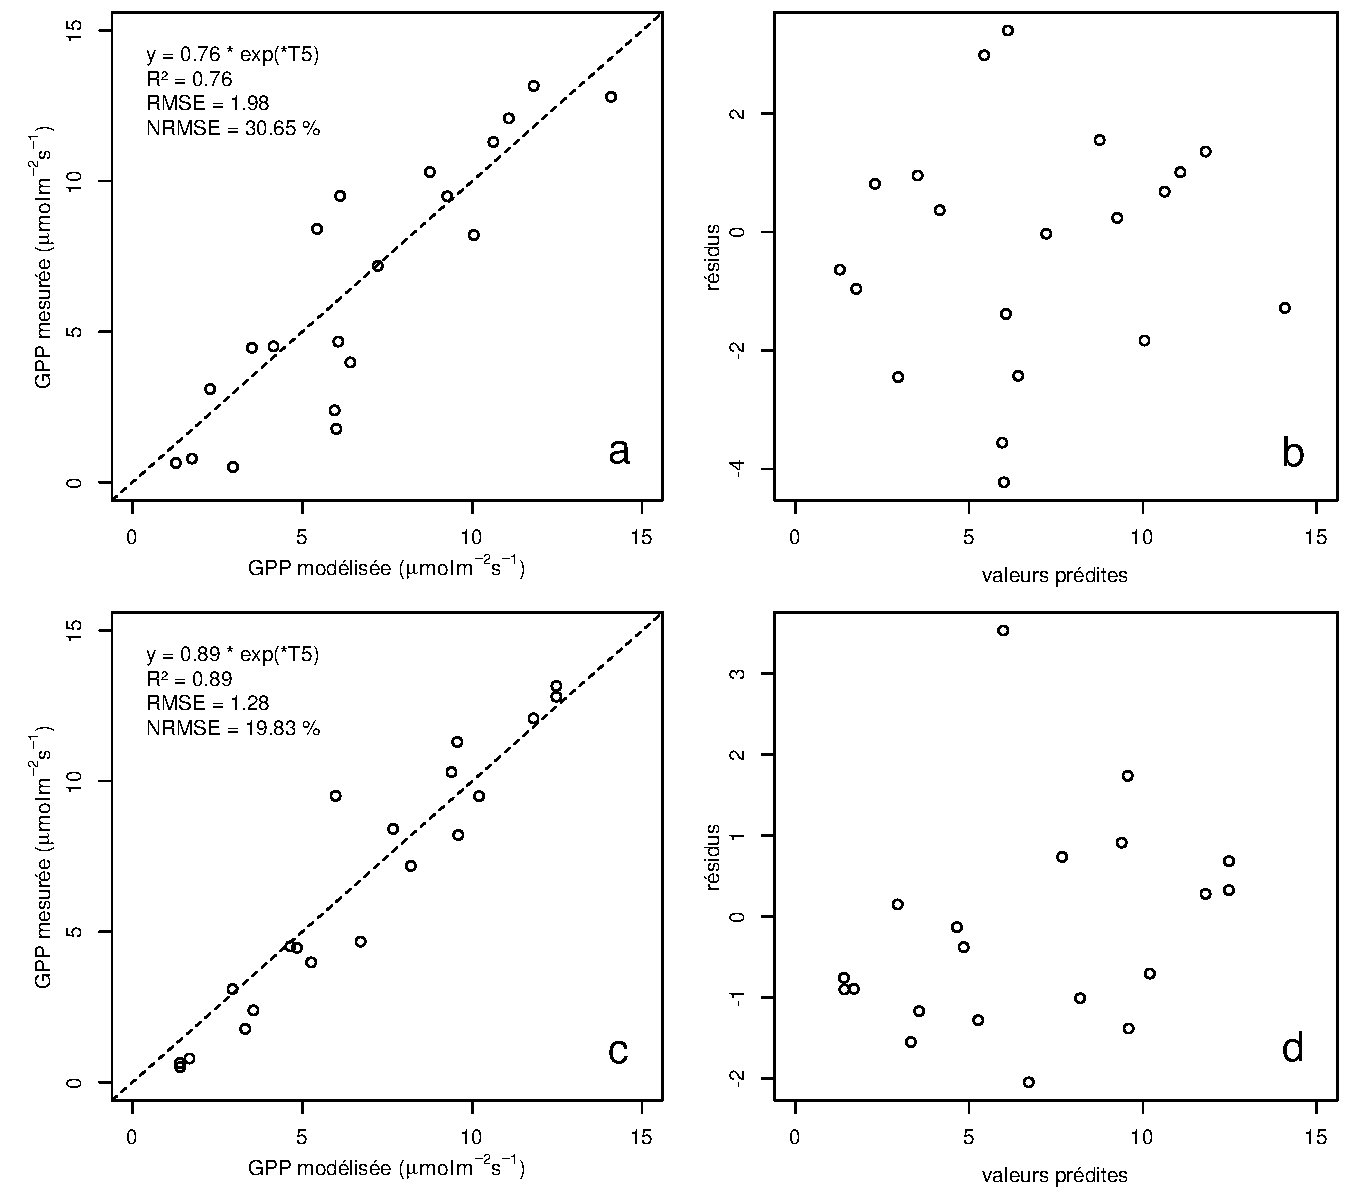
\includegraphics[width=\textwidth]{chap3/GPP_mdl_mesmod}
%\caption{PPB modèles Tair}
%\label{fig:PPB_Tair_mdl}
%\end{figure}

%La PPB calculée à partir de l'équation~\ref{eq:juneTair} présente des résidus relativement homogène avec cependant d'avantage de points situés entre \num{-2} et \num{-4} qu'entre \num{2} et \num{4} (Figure~\ref{fig:mdl_GPP_Tair}--a,b).
%Une observation similaire peut être faire pour PPB calculé à partir de l'équation~\ref{eq:juneTairIV}, avec cependant des résidus resserrés entre \num{-2} et \num{2} et un point un peu plus extrême(Figure~\ref{fig:mdl_GPP_Tair}--c,d).

\subsubsection{La Respiration de l'Écosystème}

%%%%%%%%%%%%%%%%%%%%% RE


L'estimation de la RE s'effectue avec l'équation :

\begin{equation} \label{eq:RE_T}
RE = a*exp(b*T)
\end{equation}

La température de l'air utilisée dans un modèle exponentiel permet d'expliquer \SI{90}{\percent} des variations de la respiration de l'écosystème avec une erreur standard de \SI{18}{\percent} (Figure~\ref{fig:mdl_ER_Tair}--a).
Les résidus de cette équation semblent répartis de façon non-biaisée, pas de tendance dans le nuage de point (Figure~\ref{fig:mdl_ER_Tair}--b).
L'évaluation de ce modèle montre une erreur standard de \SI{35}{\percent} avec une tendance à sous-estimer les valeurs mesurées.
Une légère tendance, moins claire que pour la PPBsat, est visible entre les résidus et l'indice de végétation ainsi qu'avec le recouvrement de la strate herbacée.
Très souvent utilisée, la température à \SI{-5}{\centi\metre} donne des résultats proche mais moins bons notamment avec une hétéroscédasticité des résidus (\textbf{Fig Annexe ?} nope : M\&M).
%Dans les deux cas, le gain possible en ajoutant un paramètre semble limité.
On adapte l'équation~\ref{eq:RE_T} pour intégrer le signal de végétation :

\begin{equation} \label{eq:RE_TIV}
RE = (a*IV + c)*exp(b*T)
\end{equation}

\begin{equation} \label{eq:RE_TH}
RE = (a*H + c)*exp(b*T)
\end{equation}

Les calibrations de ces nouvelles équations sont présentées dans la figure~\ref{fig:mdl_ER_Tair}-a,b et \ref{fig:mdl_ER_Tair}-d,e respectivement.
Dans les deux cas, l'erreur diminue pour avoisiner \SI{13}{\percent}, avec des résidus qui se répartissent de façon non-biaisée.
L'évaluation de ces deux équations montre cependant des différences :
D'un côté l'équation~\ref{eq:RE_TIV} ne permet pas de diminuer l'erreur standard qui vaut \SI{34}{\percent}, et est donc très proche des \SI{35}{\percent} calculé pour l'évaluation du modèle n'intégrant pas la végétation.
De l'autre l'évaluation de l'équation~\ref{eq:RE_TH} montre une erreur standard plus faible s'établissant à \SI{23}{\percent}.
Les paramètres des différentes équations sont présentés dans le tableau~\ref{table:mdl_par}, les modèles RE-1, RE-2, et RE-3 correspondent respectivement aux équations~\ref{eq:RE_T}, \ref{eq:RE_TIV} et \ref{eq:RE_TH}.
À l'inverse de la PPB les paramètres des modèles de la RE ont, à l'exception du paramètre c du modèle RE-2, une significativité importante et une erreur standard faible.

\begin{figure}
\centering
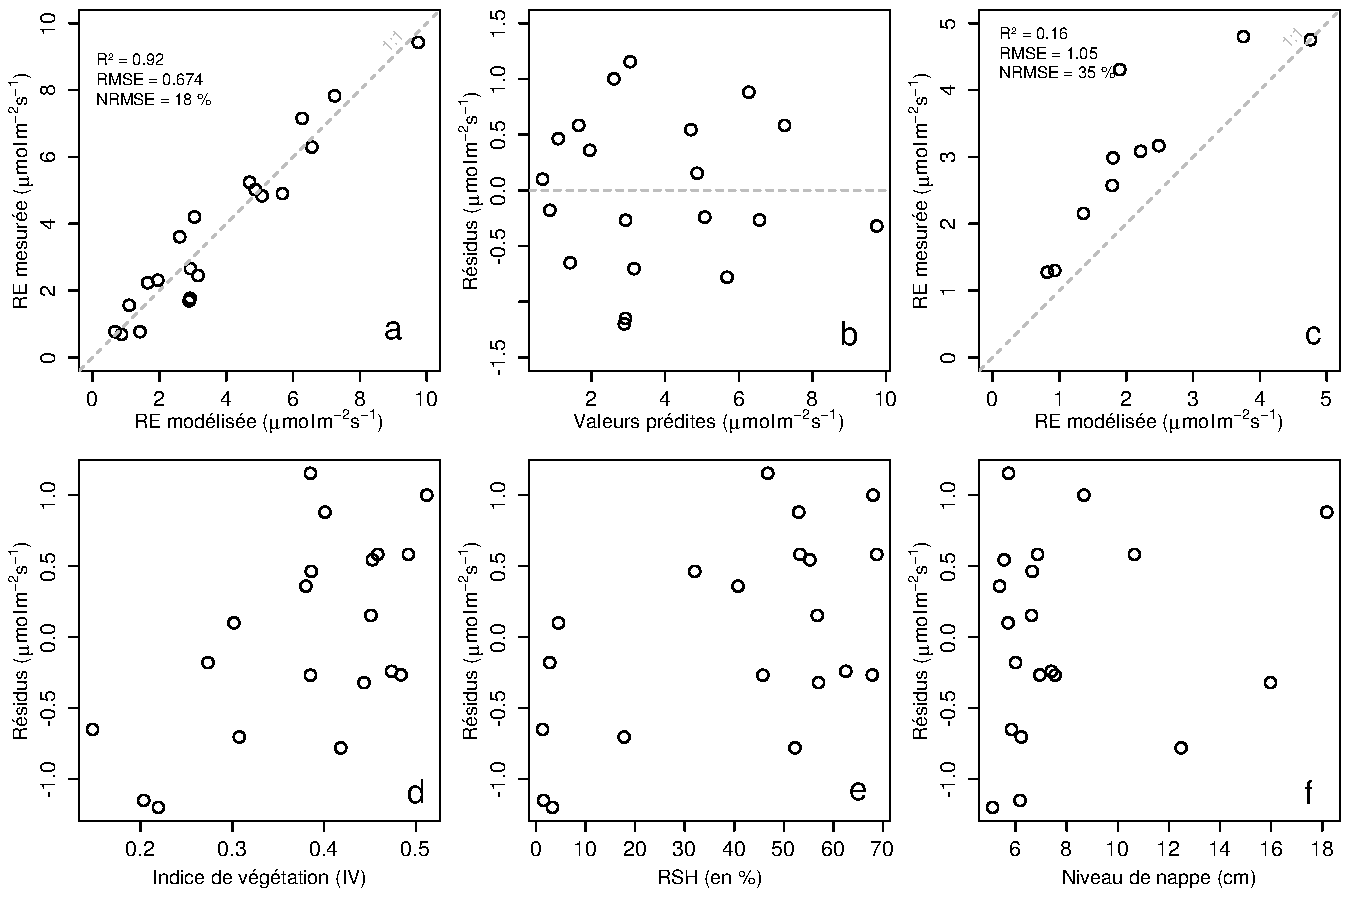
\includegraphics[width=1.05\textwidth, center]{chap3/mdl_ER_Tair}
\caption{RE modèles avec Tair}
\label{fig:mdl_ER_Tair}
\end{figure}

\begin{figure}
\centering
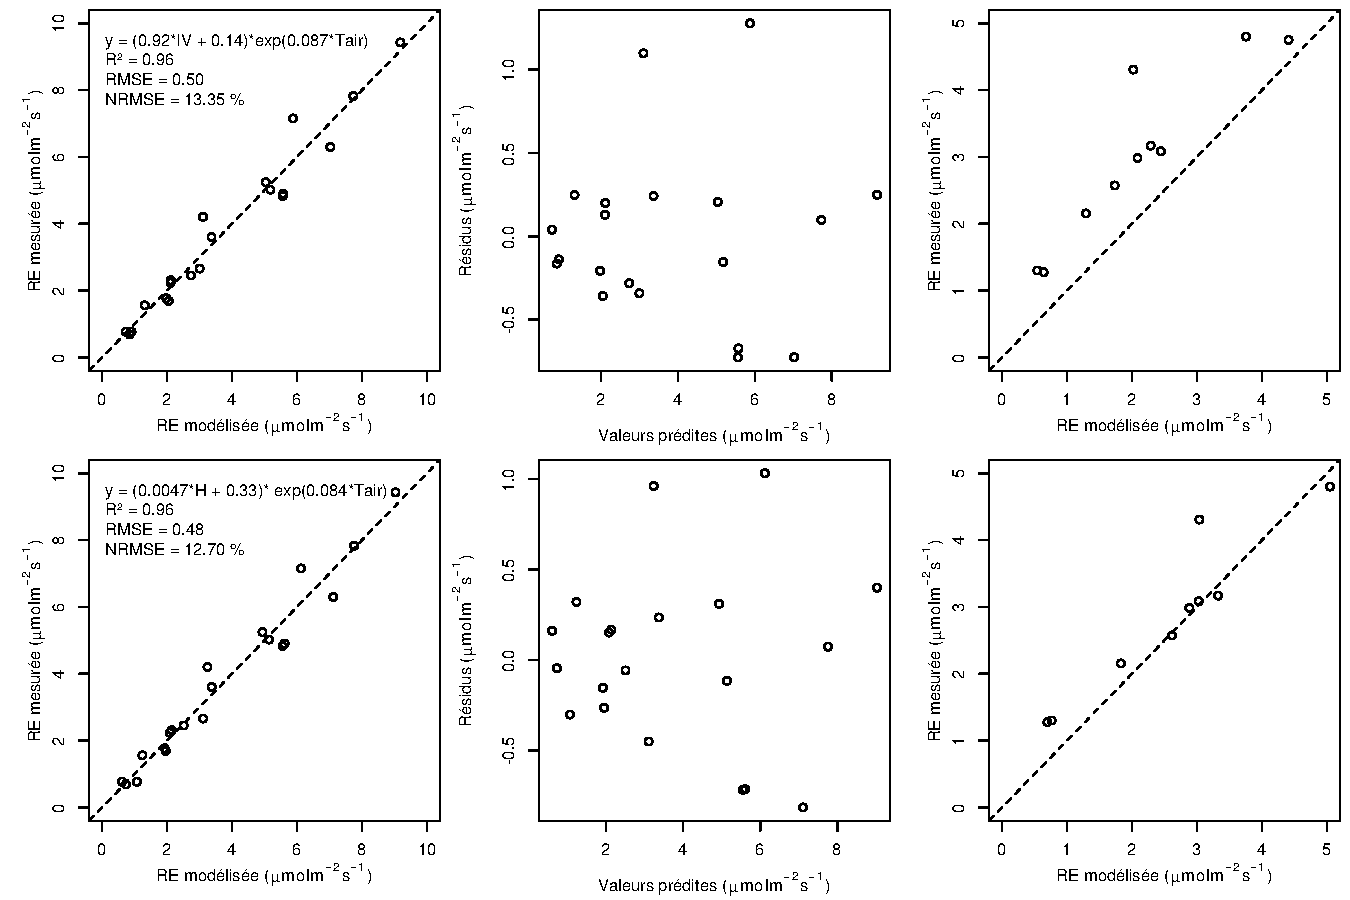
\includegraphics[width=1.05\textwidth, center]{chap3/mdl_ER_Tair_IVH}
\caption{RE modèles avec Tair}
\label{fig:ER_mdl_TairIVH}
\end{figure}

%%%%%%%%%%%%%%%%%%%%% ENE
%\subsubsection{L'Échange Net de l'Écosystème}
%
%\begin{figure}
%\centering
%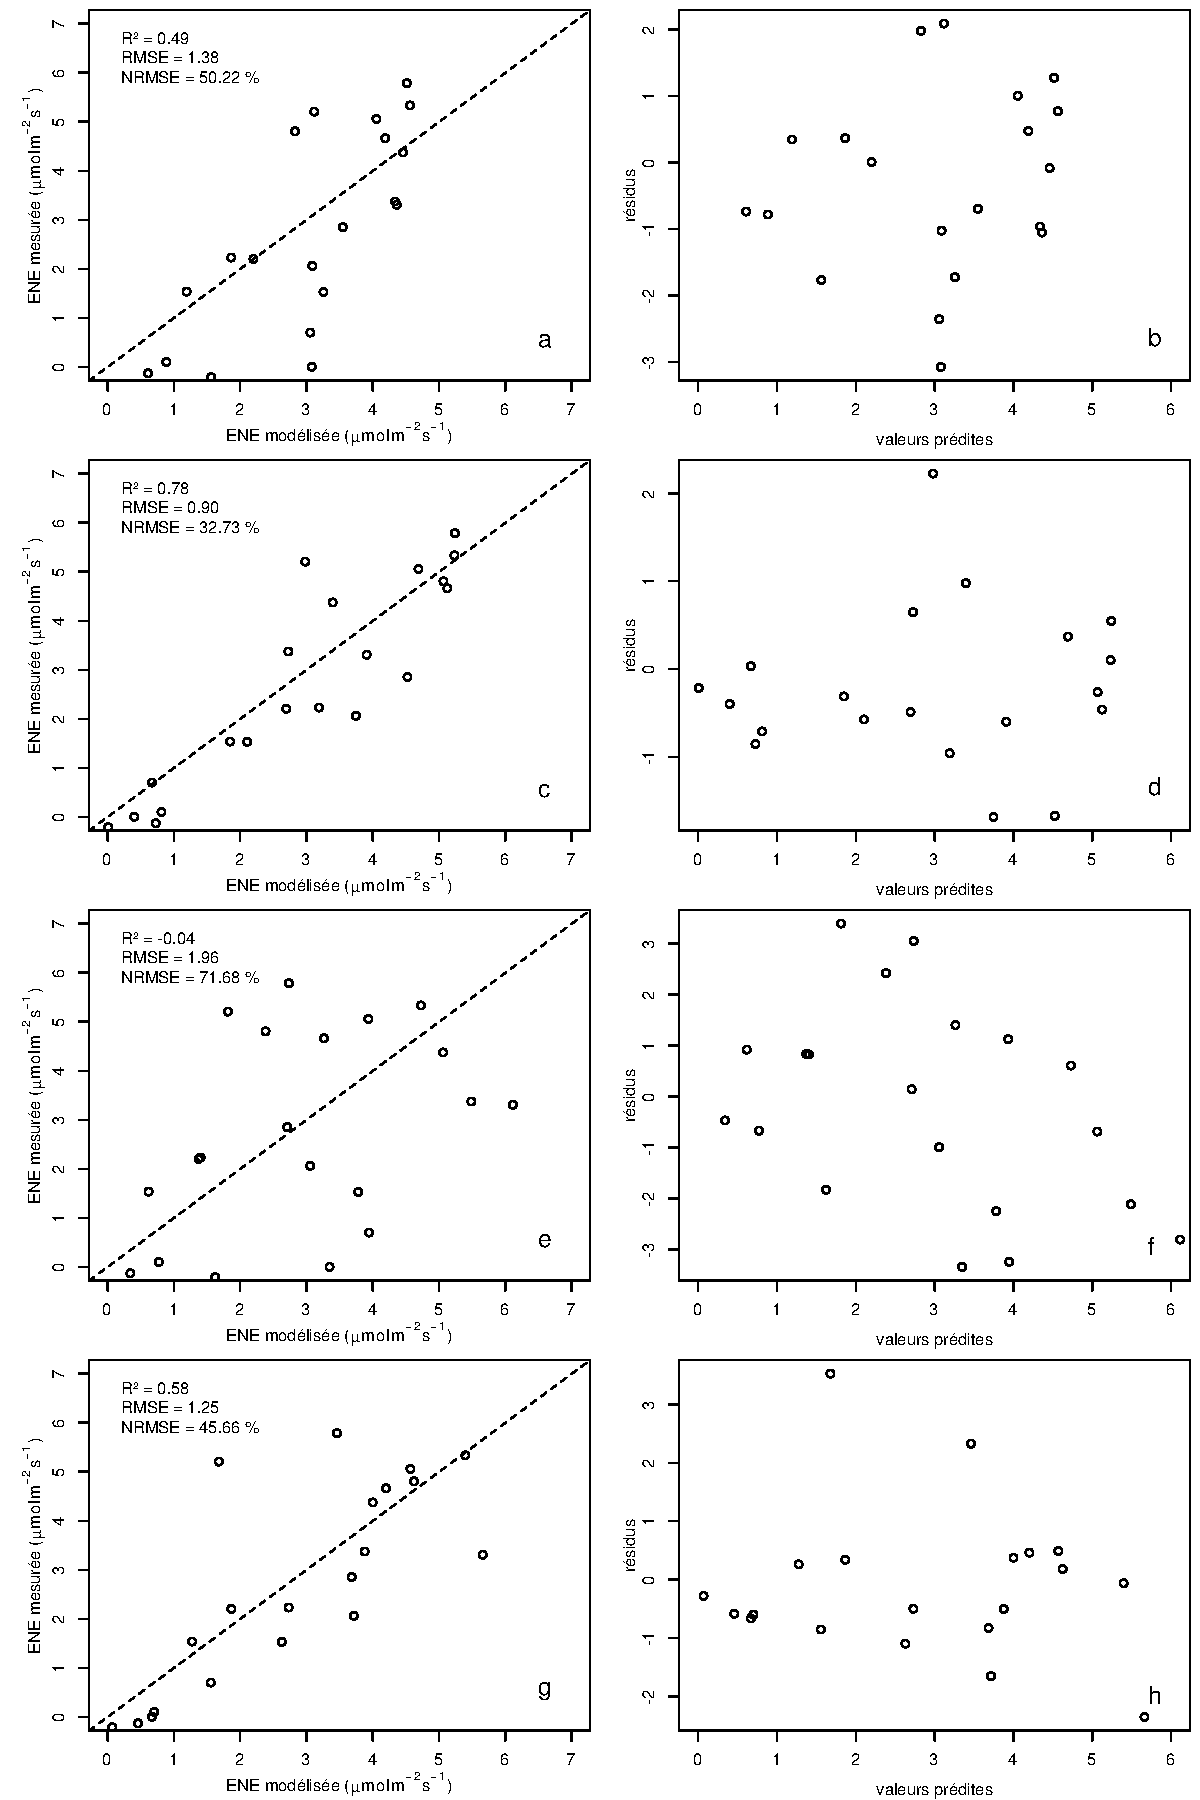
\includegraphics[width=\textwidth]{chap3/NEE_mdl_mesmod}
%\caption{ENE modèle T5 IV}
%\label{fig:ENE_mdl}
%\end{figure}
%
%L'ENE est ensuite modélisé en utilisant l'équation suivante :
%
%\begin{equation}
%ENE = PBB-RE
%\end{equation}
%
%Le résultat de cette équation (Figure~\ref{fig:ENE_mdl}), montre que ce modèle permet d'expliquer une grande partie des variations de l'ENE.
%Les résidus de cette équation sont répartis de manière a peu près homogène.

\subsubsection{Le flux de \chh}

\begin{figure}
\centering
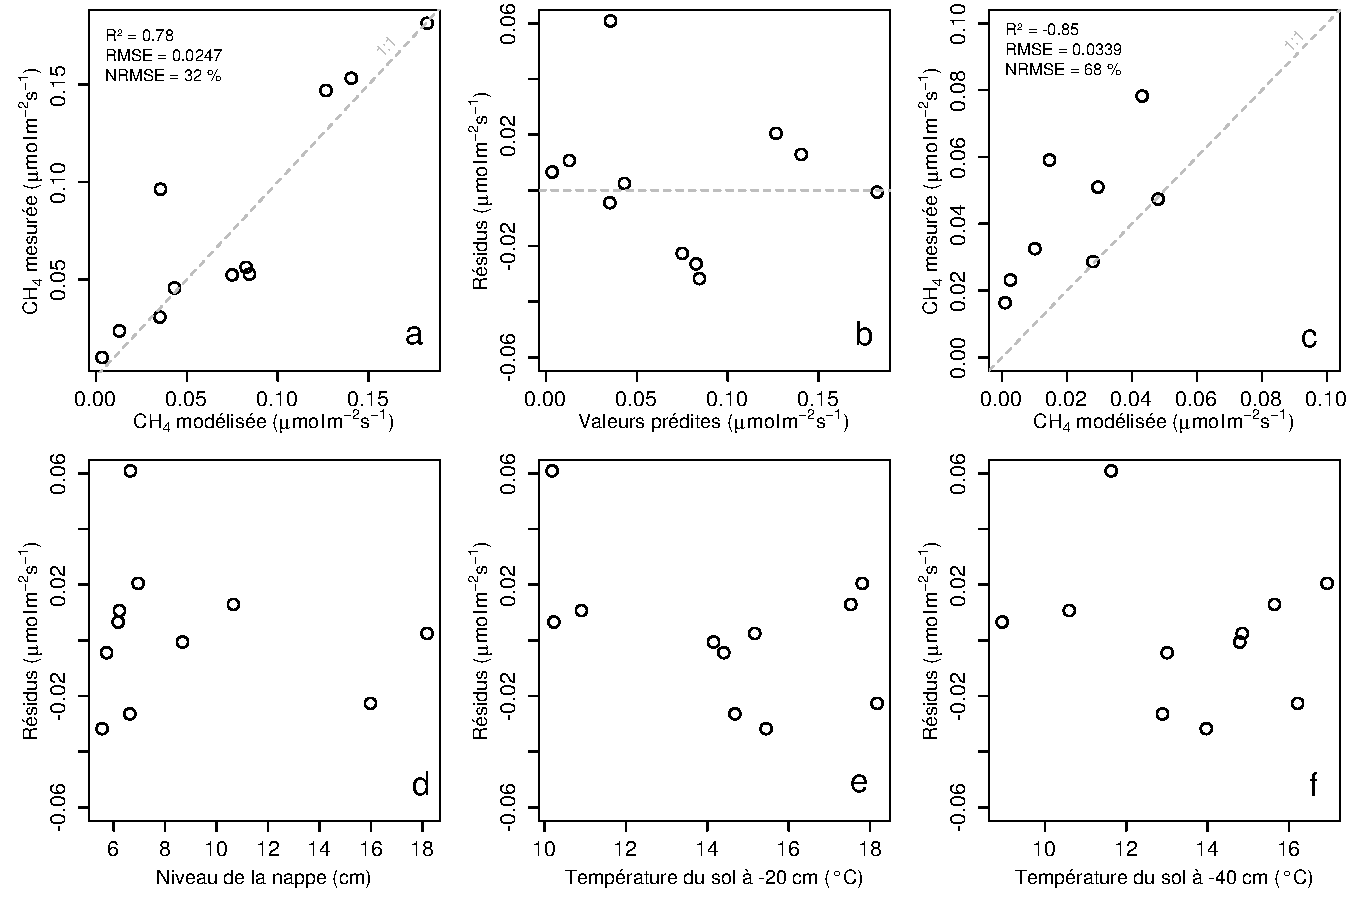
\includegraphics[width=1.15\textwidth, center]{chap3/mdl_CH4_IV}
\caption{CH4 modèle H}
\label{fig:CH4_mdl}
\end{figure}

Les relations entre les facteurs contrôlant mesurés et le \chh sont moins claires que celles concernant le \coo.
La corrélation la plus importante est liée à la végétation (R\textsuperscript{2} = \textbf{XX},Figure~\ref{fig:Fl_FC}). 
le \chh est également corrélé avec les températures, faiblement avec les températures de surface, mais de manière plus importante avec les températures du sol à plus forte profondeur (R\textsuperscript{2} = \textbf{XX},Figure~\ref{fig:Fl_FC}).
Enfin il est anti-corrélé (R=-0.51) avec le niveau de la nappe.
Les relations \chh et végétation ont donc pu être modélisées avec 

\begin{equation} \label{eq:CH4_H}
F_{CH_{4}} = a*exp(b*IV)
\end{equation}

Avec les données acquises, l'indice de végétation est le meilleur prédicteur (Figure~\ref{fig:CH4_mdl}), il explique \SI{78}{\percent} de la variabilité du \chh avec une erreur standard de \SI{32}{\percent}.
Aucune tendance ne semble se dégager entre les résidus de cette équations et les facteurs contrôlant mesurés.
L'évaluation de cette équation montre une tendance à sous-estimer les flux de \chh et une erreur standard qui double par rapport à la phase de calibration en atteignant \SI{68}{\percent}.
Les détails de l'estimation des paramètres de l'équation~\ref{eq:CH4_H} est visible dans le tableau~\ref{table:mdl_par} sous le nom FCH4.

%bortoluzzi veg
%Alm 1999 T -30 cm
%Bellisario relation inverse avec WTL (increased flux with lower WTL) T10
%Bubier 1993a WTL majeur
%Bubier 1995 Température humidité végétation

\begin{table}
\centering
\caption{Valeur des paramètres des équations utilisées pour modéliser les flux et sensibilité relative (en \%) des flux en réponse à une variation de $\pm$\SI{10}{\percent} de chacun des paramètres des modèles.}
\label{table:mdl_par}
\begin{tabular}{llccccc}\toprule

& par & valeur & se & pval & \SI{-10}{\percent} & +\SI{+10}{\percent} \\ \midrule
\multicolumn{7}{l}{PPB-1 -- équations~\ref{eq:juneTair} et \ref{eq:PPB_bubier}}  \\ [+.5ex]
& a & 26.23 & 62.07 & 0.68 & -9.7 & +9.6 	\\
& b & 53.68 & 61.27 & 0.39 & +43.7 &-35.1 \\
& c & 27.21 & 28.56 & 0.35 &-22.5 & +21.9 \\
& i &  1.84 & 21.6  & 0.93 & -0.4 &  +0.4 \\[+1ex]
\multicolumn{7}{l}{PPB-2 -- équations~\ref{eq:juneTairIV} et \ref{eq:PPB_bubier}}  \\ [+.5ex]
& a & 39.44 & 18.89 & 0.05 & -11.8 & +11.5 \\
& b & 40.27 & 19.11 & 0.05 & +15.8 & -17.2 \\
& c & 25.23 & 14.35 & 0.1 & -8.1 & +6.7 \\
& d & -3.73 & 3.49 & 0.3 & +2.8 & -2.8 \\
& i &  0.26 & 0.25 & 0.31 & -1.3 & +1.1 \\[+1ex]
\multicolumn{7}{l}{RE-1 -- équation~\ref{eq:RE_T}}  \\ [+.5ex]
& a & 0.34 & 0.08 & 0 & -10 & +10 \\
& b & 0.10 & 0.01 & 0 & -22.6 & +29.9  \\[+1ex]
\multicolumn{7}{l}{RE-2 -- équation~\ref{eq:RE_TIV}}  \\ [+.5ex]
& a & 0.92 & 0.34 & 0.02 & -7.3 & +7.3 \\
& b & 0.09 & 0.01 & 0.00 & -19.5 & 24.7 \\
& c & 0.14 & 0.09 & 0.14 & +2.7 & -2.7  \\[+1ex]
\multicolumn{7}{l}{RE-3 -- équation~\ref{eq:RE_TH}}  \\ [+.5ex]
& a & 0 & 0 & 0.01 & -3.9 & +3.9 \\
& b & 0.08 & 0.01 & 0 & -18.8 & +23.6 \\
& c & 0.33 & 0.06 & 0 & -6.1 & +6.1 \\[+1ex]
\multicolumn{7}{l}{FCH4 -- équation~\ref{eq:CH4_H}}  \\ [+.5ex]
& a & 0 & 0 & 0.48 & -10 & +10 \\
& b & 13.01 & 2.82 & 0 & -43.9 & +79.2 \\[+1ex]
\bottomrule
\end{tabular}
\end{table}


\subsubsection{Le COD}


\subsection{Le bilan de carbone de la tourbière de La Guette à l'échelle de l'écosystème}

%\subsubsection{Bilan (param et valeur)}

\begin{figure}
\centering
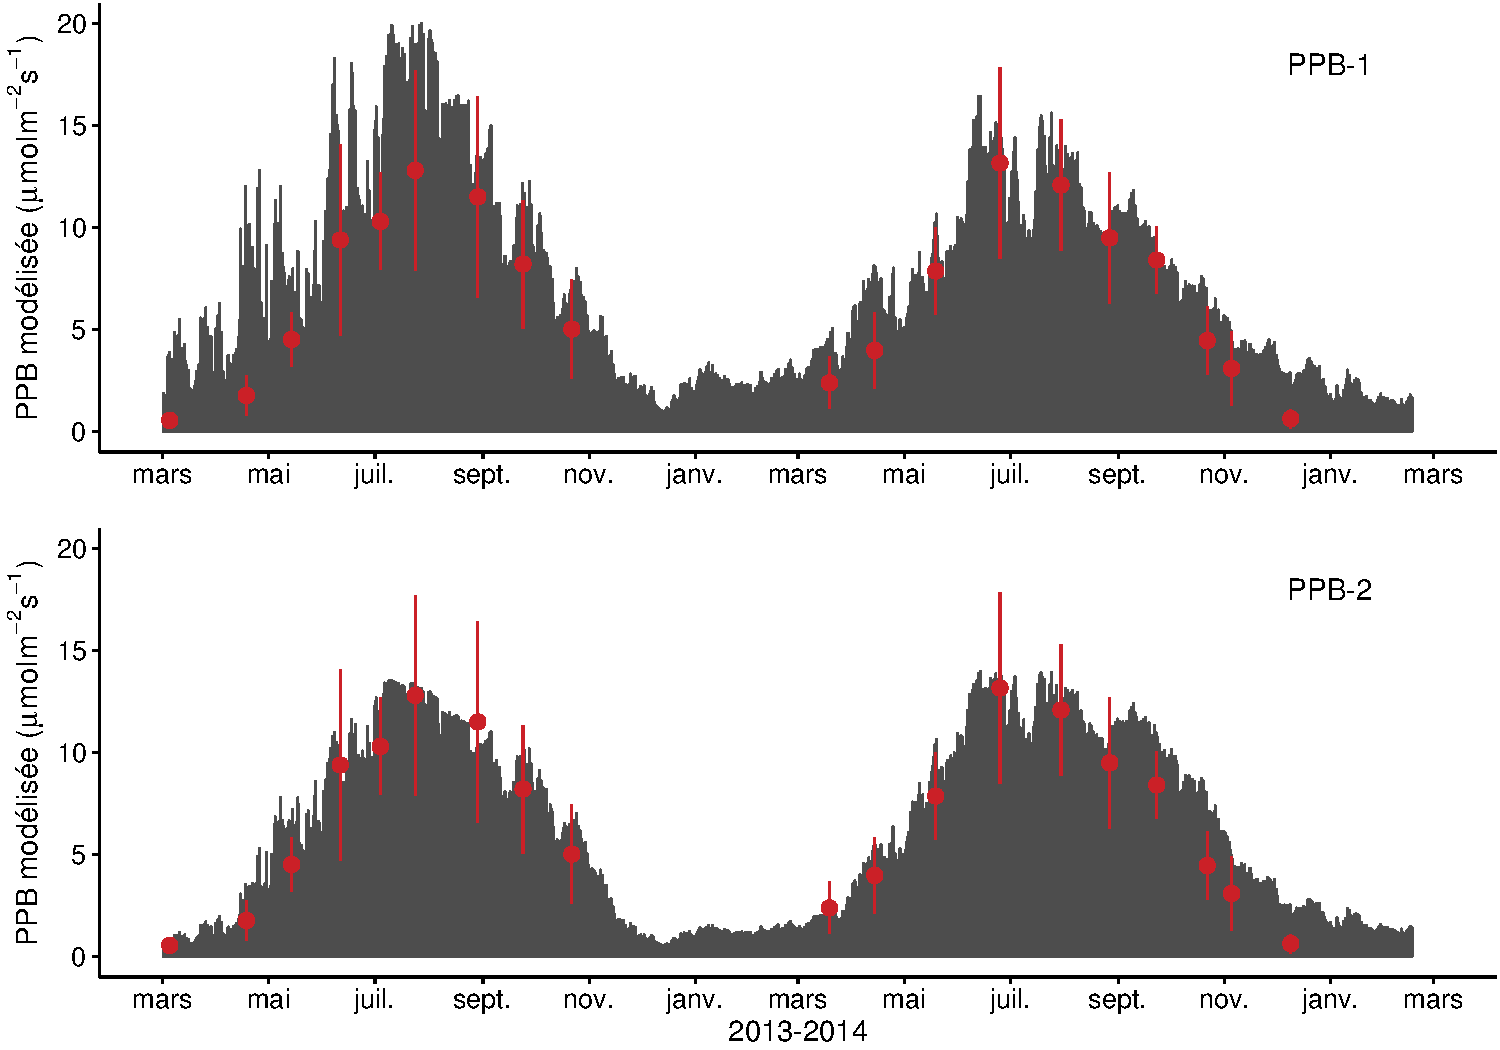
\includegraphics[width=\textwidth]{chap3/BdC_GPP_interp}
\caption{Flux de \coo interpolé à partir de PPB-1 et PPB-2}
\label{fig:BdC_GPP_interp}
\end{figure}

\begin{figure}
\centering
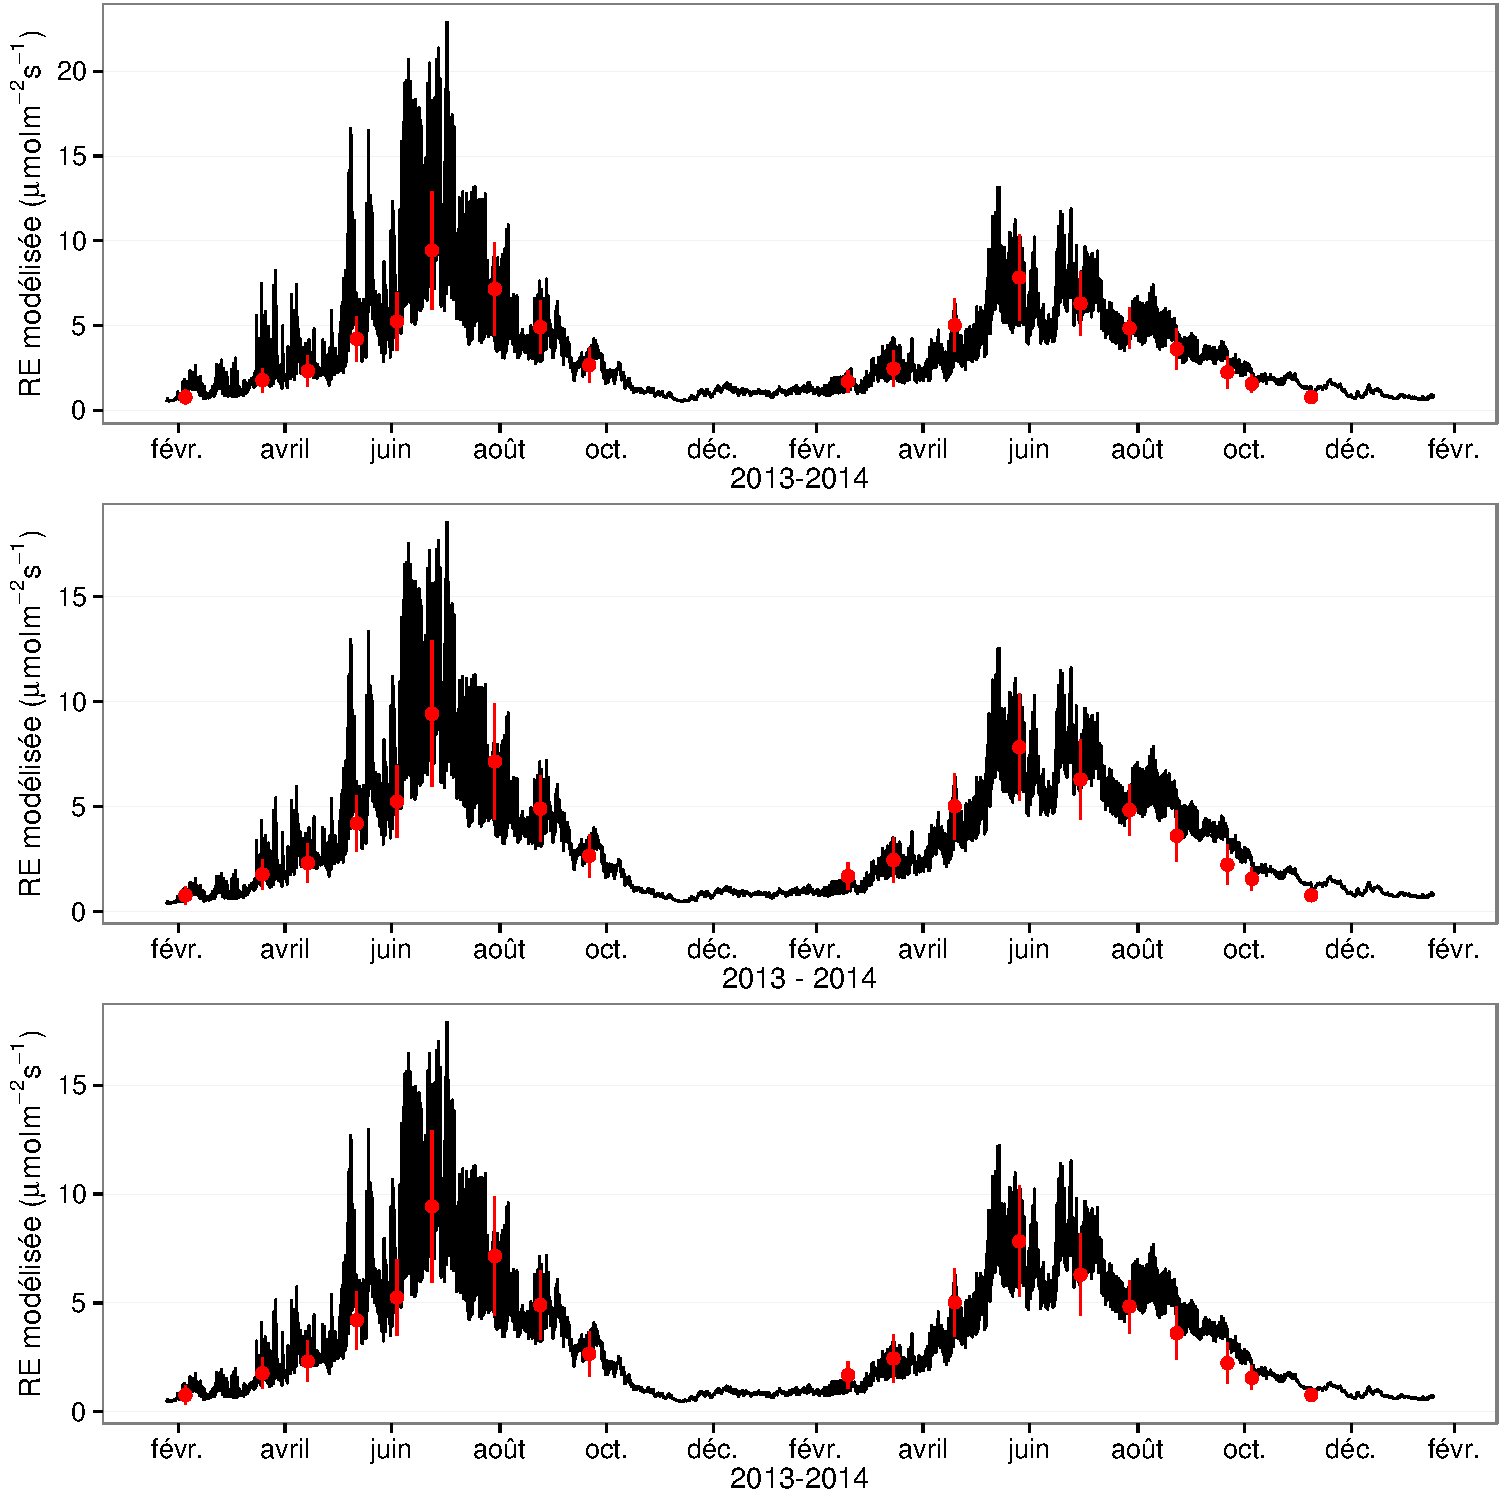
\includegraphics[width=\textwidth]{chap3/BdC_ER_interp}
\caption{Flux de \coo interpolé à partir de RE-1, RE-2 et RE-3}
\label{fig:BdC_ER_interp}
\end{figure}

\begin{figure}
\centering
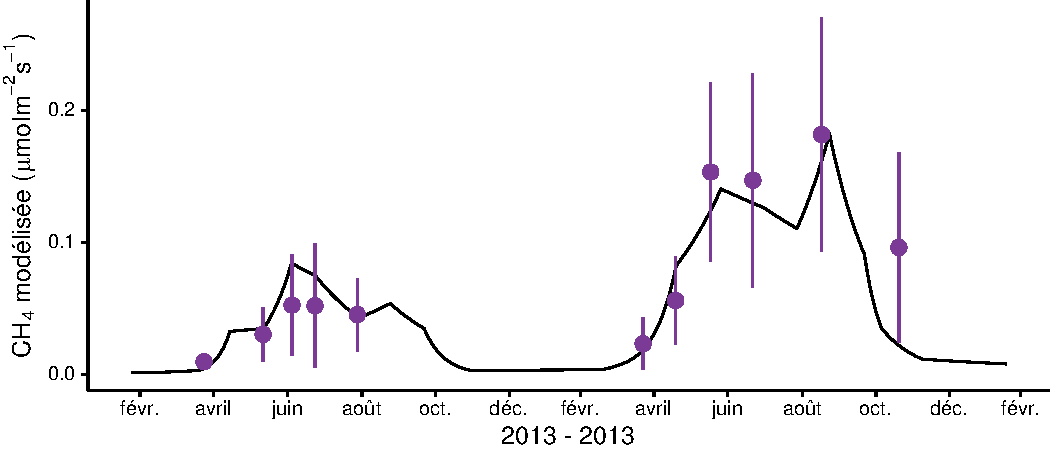
\includegraphics[width=\textwidth]{chap3/CH4_BdCitp_IVcov}
\caption{Flux de \coo interpolé à partir de RE-1, RE-2 et RE-3}
\label{fig:BdC_CH4_interp}
\end{figure}



L'interpolation des flux de PPB montrent une variabilité saisonnière proche de celle mesurée sur le terrain (Figure~\ref{fig:BdC_GPP_interp}). 
Les valeurs mesurées les plus grandes (partie supérieure de la barre rouge sur la figure~\ref{fig:BdC_GPP_interp}) ne semblent pas atteinte par le modèle PPB-2 à l'inverse du modèle PPB-1 (courbes noires sur la figure~\ref{fig:BdC_GPP_interp}).
Dans les deux cas les modèles semblent sur-estimer la valeur de PPB mesurées fin 2014.

Pour la RE, l'interpolation suit également les variations saisonnières mesurées mensuellement (Figure~\ref{fig:BdC_ER_interp}).
Les gammes de valeurs mesurées sont très proche des gammes interpolées :
les valeurs interpolées fluctuent dans les limites des barres d'erreurs.
L'interpolation des flux de la RE est très proche quel que soit le modèle utilisé (Figure~\ref{fig:BdC_ER_interp}).
L'intégration de la végétation dans les modèles RE-2 et RE-3 diminue la RE maximum modélisée en 2013 par rapport au modèle RE-1.

Les flux de \chh interpolés (Figure~\ref{fig:BdC_CH4_interp}), suivent également une cyclicité saisonnière.
L'estimation du \chh semble rendre compte dans les grandes lignes de la différence de flux mesurée entre 2013 et 2014.


%Enfin pour l'ENE, les valeur interpolées suivent les variations saisonnière, malgré une interpolation qui semble sous-estimer les flux par rapport aux valeurs mesurées (Figure~\ref{fig:BdC_interp}-c).

%\begin{table}
%\centering
%\caption{Bilan en gCm2an1}
%\label{table:BdC}
%\begin{tabular}{lllllll}\toprule
%& année & PBB & RE & CH4 & COD & BCNE \\ \midrule
%%mdl 1 (Tair - Tair - IV) & 2013 & 1317.8 $\pm$ 266 & 1332.8 $\pm$ 238 & 10.1 $\pm$ 3 & & \\[+.5ex]
%%                         & 2014 & 1257.7 $\pm$  254& 1273.3 $\pm$ 228 & 24.6 $\pm$ 8 & & \\ [+1ex]
%%                         & total & 1287.7 $\pm$ 260& 1283.9 $\pm$ 229 & 17.4 $\pm$ 6& &\\[+2ex]
%mdl 2 (Tair IV - Tair - IV) & 2013 & 1035.2 $\pm$ 209  & 1332.8 $\pm$ 238 & 10.1 $\pm$ 3 & & \\[+.5ex]
%                            & 2014 & 1212.9 $\pm$ 245 & 1273.3 $\pm$ 228  & 24.6 $\pm$ 8 &  & \\ [+1ex]
%                            & total & 1124.1 $\pm$ 227 & 1283.9 $\pm$ 229  & 17.4 $\pm$ 6 & &\\[+2ex]
%%mdl 3 (Tair IV - T5 - IV) & 2013 & 1035.2 & 1358.8 & 10.1 & & \\[+.5ex]
%%                          & 2014 & 1212.9 & 1273.3 & 24.6 & & \\ [+1ex]
%%                          & total & 1124.1 & 1288.6 & 17.4 & &\\[+1ex]
%\bottomrule
%\end{tabular}
%\end{table}


Les flux interpolés à l'heure puis sommés par années sont présentés dans le tableau~\ref{table:flux} pour les différents modèles.
Sur les deux années, selon le modèle utilisé, le flux total entrant via la PPB est estimé à 1070 et \SI{1290}{\gcma} pour PPB-2 et PPB-1 respectivement.
Dans le détail on observe une différence entre les deux modèles : 
Celui utilisant uniquement la température de l'air (PPB-1) présente un stockage plus important en 2013 qu'en 2014.
Tandis que le modèle prenant en compte la végétation (PPB-2) stocke moins de carbone en 2013 qu'en 2014.
L'intégration de la végétation minimise également l'erreur standard de l'estimation, la divisant approximativement par deux.

La différence de comportement, entre les années de mesures, liée à l'intégration de la végétation est également visible sur l'estimation de la RE.
La prise en compte de la végétation (modèles RE-2 et RE-3) conduit à une respiration plus forte en 2014 qu'en 2013 à l'inverse de RE-1.
La différence entre l'estimation de la RE en 2013 et en 2014 diminue avec l'intégration de la végétation.
Elle passe de 102 pour RE-1 à 78 puis 41 pour RE-2 et RE-3.
Malgré ces différences, on observe une grande proximité dans les valeurs des flux interpolés sur les 2 années, quel  que soit le modèle, avec un écart maximum de \SI{25}{\gcma}.

Les flux de \chh estimés ont une erreur importante et sont beaucoup plus faible que les flux de la PPB ou de la RE.
Le flux de \chh est au moins deux fois plus important en 2014 qu'en 2013.
%On y observe malgré tout un flux qui fait plus que doubler en 2014 par rapport à 2013.

Les bilans issus des différentes combinaisons de modèles (à l'exception de RE-3, non présenté car très proche de RE-2) varient de \SI{-233}{\gcma} à +\SI{12}{\gcma} stocké dans la tourbière (tableau~\ref{table:bdc}).
L'intégration de la végétation dans la modélisation de PPB fait baisser les bilans de carbone dans le négatif (système source) au-delà de \SI{-200}{\gcma}, avec une différence entre les bilans de \SI{220}{\gcma} environ.
La différence sur les bilans quand les modèles de RE utilisent ou non la végétation est moindre : environ \SI{26}{\gcma} (tableau~\ref{table:bdc}).

\begin{table}
\centering
\caption{Bilan des flux en gCm2an1}
\label{table:flux}
\begin{tabular}{llllll}\toprule
ID & Flux & équation & 2013 & 2014 & moyen \\ \midrule
PPB-1 & PPB & \ref{eq:juneTair} et \ref{eq:PPB_bubier} & 1322 $\pm$ 410 & 1258 $\pm$ 390 & 1290 $\pm$ 400 \\
PPB-2 & & \ref{eq:juneTairIV} et \ref{eq:PPB_bubier} & 957 $\pm$ 182 & 1184 $\pm$ 225 & 1070 $\pm$ 203 \\[+1.5ex]
RE-1 & RE & \ref{eq:RE_T} & 1337 $\pm$ 241 & 1235 $\pm$ 222 & 1286 $\pm$ 231 \\
RE-2 & & \ref{eq:RE_TIV} & 1232 $\pm$ 160 & 1310 $\pm$ 170 & 1271 $\pm$ 165\\
RE-3 & & \ref{eq:RE_TH} & 1240 $\pm$ 161 & 1281 $\pm$ 167 & 1261 $\pm$ 164 \\[+1.5ex]
FCH4 & CH4 & \ref{eq:CH4_H} & 10 $\pm$ 3 & 24 $\pm$ 8 & 17 $\pm$ 5 \\
\bottomrule
\end{tabular}
\end{table}


\begin{table}
\centering
\caption{Bilan des flux en gCm2an1}
\label{table:bdc}
\begin{tabular}{llll}\toprule
combinaison de modèles & 2013 & 2014 & moyen \\ \midrule
PPB-1, RE-1, FCH4 &  \num{-25} & \num{-2} & \num{-14} \\
PPB-1, RE-3, FCH4 &  +\num{72} & \num{-48} & +\num{12} \\
PPB-2, RE-1, FCH4 &  \num{-390} & \num{-75} & \num{-233} \\
PPB-2, RE-3, FCH4 &  \num{-293} & \num{-122} & \num{-208} \\
\bottomrule
\end{tabular}
\end{table}


\subsubsection{Évaluation du bilan}

%\subsubsection{sensibilité des paramètres}
\begin{table}
\centering
\caption{Sensibilité relative (en \%) du bilan de \coo (ENE) en réponse à une variation de $\pm$\SI{10}{\percent} de chacun des paramètres des modèles.}
\label{table:mdl_sensitiv_BdC}
\begin{tabular}{cccccccccc}\toprule
& \multicolumn{3}{l}{PPB} & \multicolumn{3}{l}{RE} & \multicolumn{3}{l}{\chh} \\ 
& & \SI{-10}{\percent} & +\SI{+10}{\percent} & & \SI{-10}{\percent} & +\SI{+10}{\percent} & & \SI{-10}{\percent} & +\SI{+10}{\percent} \\ \midrule
& \multicolumn{3}{l}{PPB-1} & \multicolumn{3}{l}{RE-1} & \multicolumn{3}{l}{FCH4} \\ [+.5ex]
& a & \num{-3263} & +\num{3243} & a & +\num{3371} & \num{-3371} & a & +\num{0.05} & \num{-0.05}\\
& b & +\num{14788} & \num{-11859} & b & +\num{7616} & \num{-10078} & b & +\num{0.2} & \num{-0.36}\\
& c & \num{-7597} & +\num{7398} & & & & & &\\
& i & +\num{119} & \num{-139} & & & & & &\\[+1ex]

& \multicolumn{3}{l}{PPB-2} & \multicolumn{3}{l}{RE-1} & \multicolumn{3}{l}{FCH4} \\ [+.5ex]
& a & +\num{59} & \num{-57} & a & \num{-60} & +\num{60} & a & \num{0} & \num{0}\\
& b & \num{-78} & +\num{85} & b & \num{-135} & +\num{178} & b & \num{0} & +\num{0.01}\\
& c & +\num{40} & \num{-33} & & & & & &\\
& d & \num{-14} & +\num{14} & & & & & &\\
& i & \num{6.22} & \num{-5.40} & & & & & &\\[+1ex]

& \multicolumn{3}{l}{PPB-1} & \multicolumn{3}{l}{RE-3} & \multicolumn{3}{l}{FCH4} \\ [+.5ex]
& a & \num{-426} & +\num{423} & a & +\num{168} & \num{-168} & a & +\num{0.01} & \num{-0.01}\\
& b & +\num{1931} & \num{-1548} & b & +\num{813} & \num{-1018} & b & +\num{0.03} & \num{-0.05}\\
& c & \num{-992} & +\num{966} & c & +\num{263} & \num{-263} & & &\\
& i & \num{-18} & +\num{15} & & & & & &\\[+1ex]

& \multicolumn{3}{l}{PPB-2} & \multicolumn{3}{l}{RE-3} & \multicolumn{3}{l}{FCH4} \\ [+.5ex]
& a & +\num{67} & \num{-65} & a & \num{-26} & +\num{26} & a & 0 & 0\\
& b & \num{-89} & +\num{97} & b & \num{-125} & +\num{157} & b & 0 & 0\\
& c & +\num{45} & \num{-38} & c & \num{-40} & +\num{40} & & &\\
& d & \num{-16} & +\num{16} & & & & & &\\
& i & +\num{7.1} & \num{-6.1} & & & & & &\\[+1ex]

\bottomrule
\end{tabular}
\end{table}

L'analyse de sensibilité, consistant à faire varier chaque paramètre des modèles de $\pm$\SI{10}{\percent}, les combinaisons de modèles PPB-1, PPB-2, RE-1 et RE-3 ont été testé (Tableau~\ref{table:mdl_sensitiv_BdC}).
Le modèle RE-2, très proche du modèle RE-3 n'a pas été testé.
\textbf{Attente du COD, les valeurs du tableau sont fausse pour le moment}

%, montre pour une équation exponentielle simple des valeurs attendues $\pm$\SI{10}{\percent} pour le paramètre a et \num{+29} à \SI{-22}{\percent} pour le b (Figure~\ref{table:mdl_sensitiv}).
%Pour la PPB issue des équations~\ref{eq:juneTairIV} et \ref{eq:PPB_bubier} le paramètre i à très peu d'effet sur le bilan, \num{0} à \SI{-1}{\percent}.
%Cependant l'effet sur le bilan augmente lorsque la végétation est prise en compte (équation~\ref{eq:juneTair} et \ref{eq:PPB_bubier}) : \num{-8} à \SI{-10}{\percent}.
%À l'inverse, la sensibilité de l'ensemble des autres paramètres (a, b, c) diminue lorsque l'indice de végétation est pris en compte.
%Le paramètre a est l'exception, passant de \num{-10} à \SI{-17}{\percent} pour une baisse de \SI{10}{\percent}.
%Considérant le modèle de PPB prenant en compte la végétation, la sensibilité maximum des différents paramètres du bilan est proche de \SI{30}{\percent}, et similaire pour la PPB et la RE.



%\begin{table}
%\centering
%\caption{Sensibilité relative (en \%) du bilan de \coo (ENE) en réponse à une variation de $\pm$\SI{10}{\percent} de chacun des paramètres des modèles.}
%\label{table:mdl_sensitiv_BdC}
%\begin{tabular}{llccccccccccc}\toprule
%& \multicolumn{4}{l}{PPB} & \multicolumn{4}{l}{RE} & \multicolumn{4}{l}{\chh} \\ 
%& par & valeur & \SI{-10}{\percent} & +\SI{+10}{\percent} & par & valeur & \SI{-10}{\percent} & +\SI{+10}{\percent} & par & valeur & \SI{-10}{\percent} & +\SI{+10}{\percent} \\ \midrule
%\multicolumn{13}{l}{PPB-2, ER-3, FCH4} \\ [+.5ex]
%& a & 0.34 & -766 & 766 & a & 26.23 & 741 & -736 & a & 17.82 & -12.28 & 12.28 \\
%& b & 0.10 & -1730 & 2289 & b & 53.68 & -3358 & 2693 & b & 0.03 & -15.08 & 17.68 \\
%& c &  & & & c & 27.21 & 1725 & -1680 & & & & \\
%& d &  & & & c & 27.21 & 1725 & -1680 & & & & \\
%& e &  & & & i & 1.84 & 31.56 & -26.92 & & & & \\[+1ex]
%%\multicolumn{13}{l}{mdl 2 équation~\ref{eq:RE_T5} et équation~\ref{eq:juneTairIV} Tair, Tair IVcov, H} \\ [+.5ex]
%%& a & 0.34 & -71.08 & 71.08 & a & 33.66 & 56.25 & -55.32 & a & 17.82 & -1.14 & 1.14 \\
%%& b & 0.10 & -160.59 & 212.51 & b & 42.45 & -119.84 & 123.69 & b & 0.03 & -1.40 & 1.64 \\
%%&  &  & & & c & 25.77 & 62.63 & -53.28 & & & & \\
%%&  &  & & & i & 0.33 & 6.94 & -6.02 & & & & \\[+1ex]
%%\multicolumn{13}{l}{mdl 3 équation~\ref{eq:RE_T5IV} et équation~\ref{eq:juneTairIV} Tair IVcov, Tair IVcov, H} \\ [+.5ex]
%%& a & 0.92 & -55.69 & 55.69 & a & 33.66 & 61.31 & -60.31 & a & 17.82 & -1.24 & 1.24 \\
%%& b & 0.09 & -149.40 & 189.01 & b & 42.45 & -130.64 & 134.84 & b & 0.03 & -1.53 & 1.79 \\
%%& c & 0.14 & -20.89 & 20.89 & c & 25.77 & 68.28 & -58.08 & & & & \\
%%&  &  & & & i & 0.33 & 7.57 & -6.56 & & & & \\
%\bottomrule
%\end{tabular}
%\end{table}


%\begin{table}
%\centering
%\caption{Sensibilité relative (en \%) des flux en réponse à une variation de $\pm$\SI{10}{\percent} de chacun des paramètres des modèles.}
%\label{table:mdl_sensitiv}
%\begin{tabular}{llccccccccccc}\toprule
%& \multicolumn{4}{l}{RE} & \multicolumn{4}{l}{GPP} & \multicolumn{4}{l}{\chh} \\ 
%& par & valeur & \SI{-10}{\percent} & +\SI{+10}{\percent} & par & valeur & \SI{-10}{\percent} & +\SI{+10}{\percent} & par & valeur & \SI{-10}{\percent} & +\SI{+10}{\percent} \\ \midrule
% & \multicolumn{4}{l}{Tair} & \multicolumn{4}{l}{Tair} & \multicolumn{4}{l}{H} \\ [+.5ex]
%& a & 0.34 & -10   & 10   & a & 26.23 & -9.7 &  9.6 & a & 17.82 &-10.0 & 10.0 \\
%& b & 0.10 & -22.6 & 29.9 & b & 53.68 & 43.7 &-35.1 & b &  0.03 &-12.3 & 14.4 \\
%&   &      &       &      & c & 27.21 &-22.5 & 21.9 &   &       &      &      \\
%&   &      &       &      & i &  1.84 & -0.4 &  0.4 &   &       &      &      \\[+1ex]
% & \multicolumn{4}{l}{Tair IVcov} & \multicolumn{4}{l}{Tair IVcov} & & & & \\ [+.5ex]
%& a & 0.92 & -7.3  & 7.3 & a & 33.66 & -9.0 &  8.9 & & & & \\
%& b & 0.09 & -19.5 & 24.7& b & 42.45 & 19.3 &-19.9 & & & & \\
%& c & 0.14 & -2.7  & 2.7 & c & 25.77 &-10.1 &  8.6 & & & & \\
%&   &      &       &     & i & 0.33  & -1.1 &  1.0 & & & & \\[+1ex]
%\bottomrule
%\end{tabular}
%\end{table}




%\subsubsection{pseudo-validation et erreur}

%\begin{figure}
%\centering
%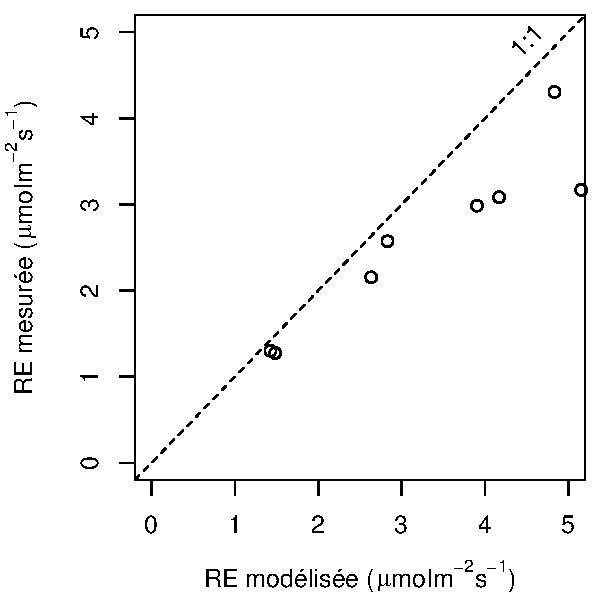
\includegraphics[width=.5\textwidth]{chap3/ER_T5_val}
%\caption{Évaluation RE}
%\label{fig:RE_T5_val}
%\end{figure}
%\begin{figure}
%\centering
%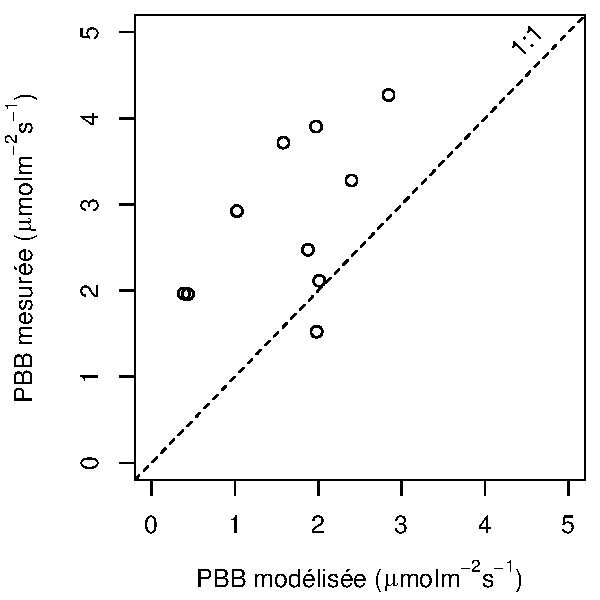
\includegraphics[width=.5\textwidth]{chap3/GPP_TairIVcov_val}
%\caption{Évaluation GPP}
%\label{fig:GPP_TairIVcov_val}
%\end{figure}

\subsection{Variabilité spatiale du bilan}

\subsubsection{Calibration par groupe de placette}



\begin{figure}
\centering
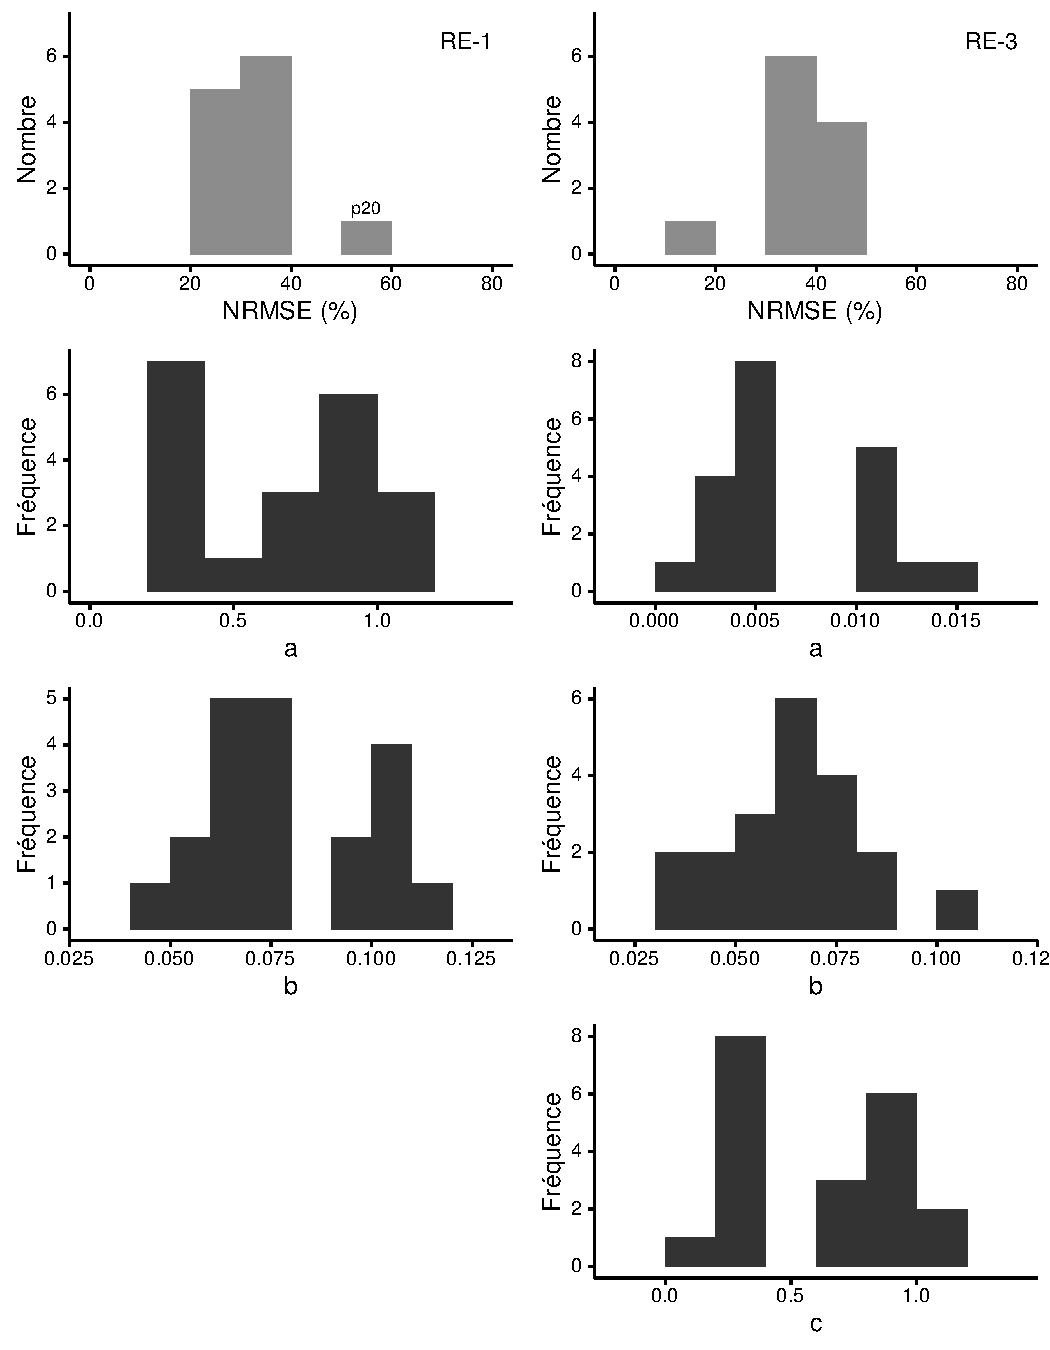
\includegraphics[width=\textwidth]{chap3/loc_ER}
\caption{Distribution de l'erreur standard (en gris) par placette et des paramètres des modèles RE-1 et RE-3 (en noir)}
\label{fig:loc_ER}
\end{figure}

\begin{figure}
\centering
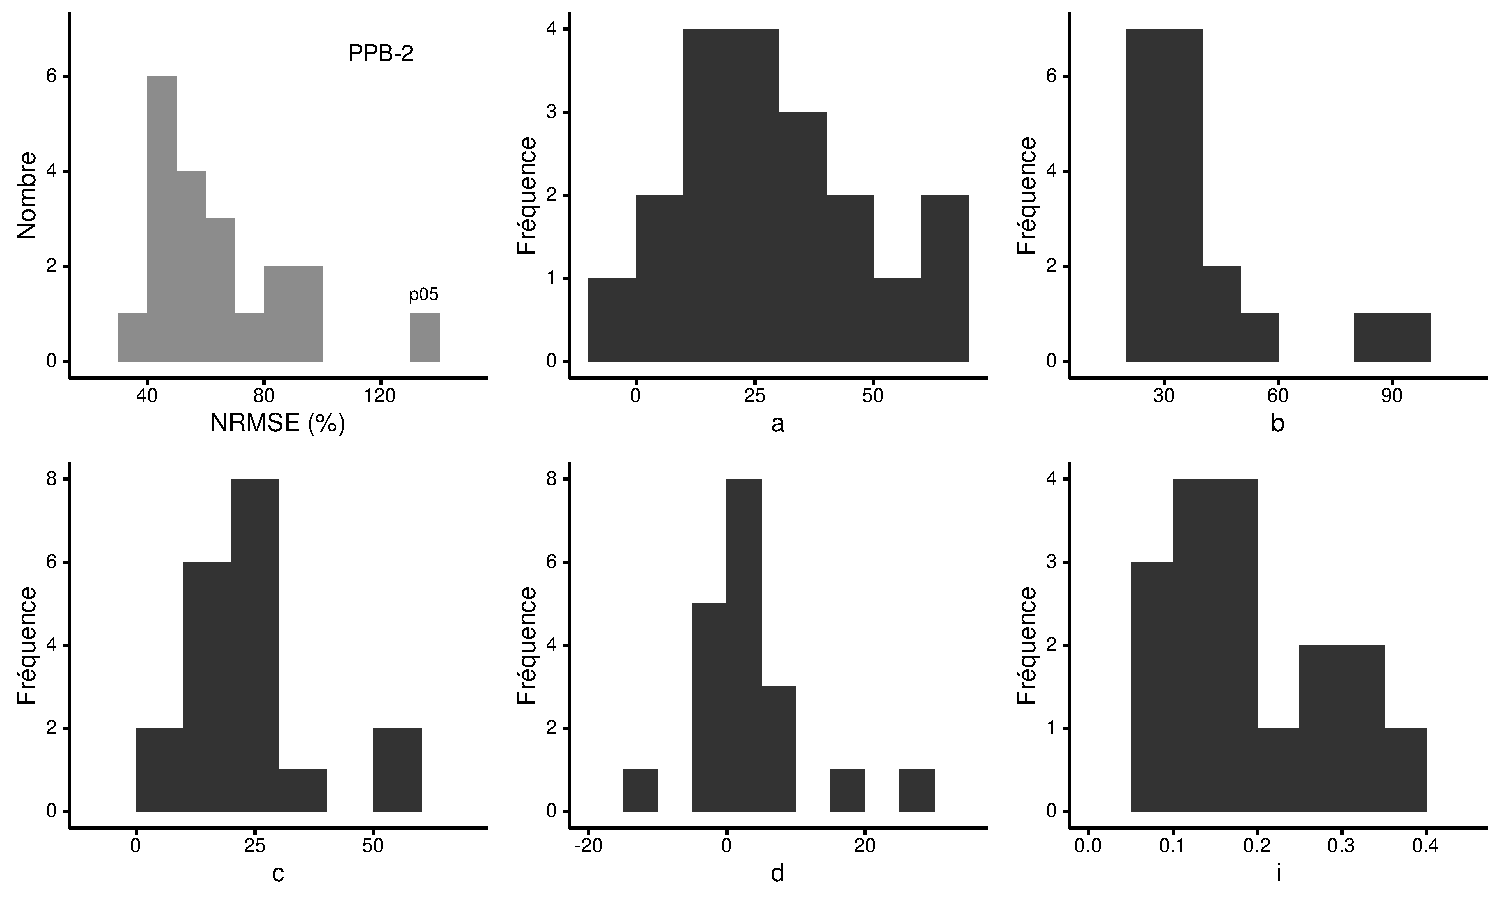
\includegraphics[width=1.15\textwidth, center]{chap3/loc_GPP}
\caption{Distribution de l'erreur standard par placette (en gris) et des paramètres du modèle PPB-2 (en noir)}
\label{fig:loc_GPP}
\end{figure}

La classification hiérarchique a permis de distinguer 4 groupes de végétation (Figure~\ref{fig:tree}).
Dans le groupe Mousse, la strate muscinale est majoritaire avec un recouvrement moyen de \SI{91}{\percent}, moins de \num{35} et \SI{15}{\percent} de recouvrement pour les herbacées et les arbustes respectivement.
Le groupe Mix est le plus homogène avec un recouvrement moyen des strates muscinales et arbustives de \num{63} et \SI{58}{\percent} chacune.
C'est également le groupe ou il y a de moins d'herbacées avec un recouvrement de \SI{24}{\percent}.
La strate herbacée est majoritaire dans le Herbe avec un recouvrement moyen de \SI{63}{\percent}, la strate arbustive y est peu présence (\SI{19}{\percent} en moyenne) et la strate muscinale y est pour ainsi dire absente (\SI{1}{\percent}).
La strate muscinale est également absente, ou presque, dans le groupe Arbuste (\SI{1}{\percent}).
Groupe dans lequel la strate arbustive est majoritaire avec de \SI{65}{\percent} de recouvrement moyen, et la strate herbacée avec \SI{33}{\percent} (Figure~\ref{fig:distrib_grpveg}).

\begin{figure}
\centering
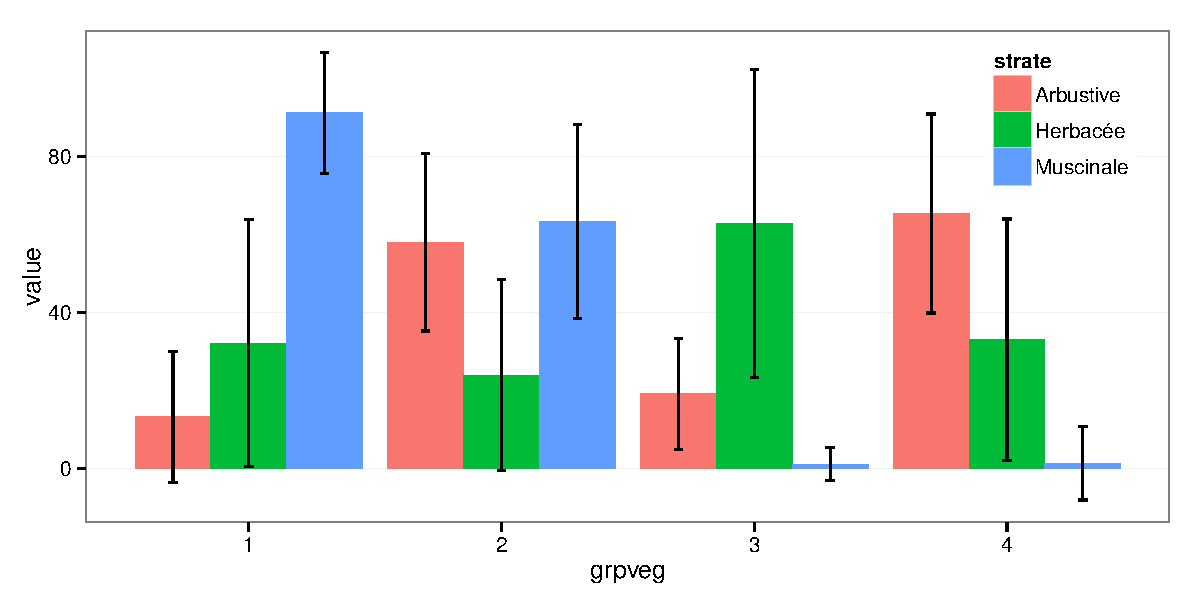
\includegraphics[width=\textwidth]{chap3/distrib_grpveg}
\caption{Recouvrement végétal moyen par strate (en \si{\percent}) des 4 groupes, les groupes sont nommés en fonction de la végétation majoritaire. Les barres d'erreur représente la déviation standard.}
\label{fig:distrib_grpveg}
\end{figure}


Les bilans de \coo calculés par groupe de végétations sont présentés dans le tableau~\ref{table:bdc_grp}.
On constante que du point de vue de l'ENE les groupes Mousse et Mix sont relativement proche, et que le groupe Arbuste est du même ordre de grandeur bien qu'avec une ENE un peu plus élevée.
Le groupe Herbe est le seul groupe présentant une ENE positive, du même ordre de grandeur que les précédentes en valeur absolue.
Dans le détail, la RE est la plus forte, supérieure à \SI{1200}{\gcma}, dans les groupes Mix et Arbuste.
Elle est plus faible dans les groupes Mousse et Herbe (environ \SI{1000}{\gcma}).
Pour la PPB, la valeur la plus faible est dans le groupe Mousse et la plus forte dans le groupe Herbe avec plus de \SI{1300}{\gcma}, soit une différence de plus de \SI{600}{\gcma}.
Les groupes Mix et Arbuste sont relativement proches avec des valeurs intermédiaires avoisinant \SI{1000}{\gcma}.

\begin{table}
\centering
\caption{Bilan des flux de \coo en \si{\gcma}, en utilisant PPB-2 et RE-3}
\label{table:bdc_grp}
\begin{tabular}{llll}\toprule
groupe & PPB-2 & RE-3 & ENE \\ \midrule
Mousse &  \num{714} & \num{1023} & \num{-308} \\
Mix &  \num{1045} & \num{1385} & \num{-340} \\
Herbe &  \num{1323} & \num{1057} & \num{266} \\
Arbuste &  \num{1002} & \num{1262} & \num{-260} \\
\bottomrule
\end{tabular}
\end{table}

\subsubsection{Calibration par placette}

Les modèles RE-1, RE-3 et PPB-2 ont pu être calibré par placette.
Pour l'ensemble de ces modèles on constate une forte hausse de la NRMSE (Figure~\ref{fig:loc_ER} et \ref{fig:loc_GPP}).
Concernant la RE, les modèles RE-1 et RE-3 ont des valeurs de NRMSE relativement proche d'environ \SI{50}{\percent}, avec deux outliers pour RE-1 et un pour RE-3 (Figure~\ref{fig:loc_ER}).
Les paramètres varient dans des gammes similaires pour les deux modèles.
Ces gammes sont larges et bien supérieure à \SI{10}{\percent}.
Concernant la PPB, le modèle PPB-2 a également une NRMSE importante, variant entre 40 et \SI{100}{\percent} avec un outlier.
Les valeurs des paramètres varient également de façon importante (Figure~\ref{fig:loc_GPP}).

\subsubsection{Corrélation avec facteurs contrôlant}

\section{Discussion}

\subsection{Estimations des flux}

\subsubsection{PPB}

% Flux mesurés // biblio
%Les flux mesurés sont ...
%
%aurela 2007 inf \SI{5}{\uml}

% Flux modélisés

L'estimation des flux de PPB, est comprise entre 957 et \SI{1322}{\gcma} selon l'année et le modèle utilisé.
Ces valeurs sont très élevées comparées à des tourbières boréales comme celles étudiées par \citep{trudeau2014} ou encore \citep{peichl2014} dont les valeurs de PPB sont respectivement comprise entre 123 et \SI{131}{\gcma} et entre 203 et \SI{503}{\gcma}.
Une première hypothèse permettant d'expliquer une telle différence, est la différence entre les températures moyennes sur les sites.
\SI{-4.3}{\degreeCelsius} et \SI{1.2}{\degreeCelsius} respectivement pour \citet{trudeau2014} et \citet{peichl2014}.
Ces températures sont bien plus faible pour les sites des études pré-citées que sur la tourbière de La Guette.
Une seconde hypothèse, qui n'exclue par la première, serait la composition végétale de ces sites. 
La tourbière de La Guette envahie par une végétation vasculaire, notamment herbacée, est plus proche d'une prairie tourbeuse que d'une tourbière boréale.
En effet les valeurs observées à La Guette sont comparables à ce type d'écosystèmes.
\citet{jacobs2007} estiment des valeurs de PPB comprises entre 400 et \SI{2000}{\gcma} avec une moyenne de \SI{1300}{\gcma} dans des prairies tourbeuses hollandaises.
Sur des écosystèmes similiaires, au Danemark, \citep{gorres2014} trouve des valeurs de PPB plus importantes encore, entre 1555 et \SI{2590}{\gcma}.
Il apparait cohérent que la tourbière de La Guette, par sa position géographique, et donc le climat qu'elle subit, mais également par sa problématique d'envahissement important par une végétation vasculaire notamment herbacée, s'approche en termes de flux de site tourbeux drainés pour les utiliser comme prairie.
%jacobs 2007  sols tourbeux 1300 $\pm$ \SI{100}{\gcma} (grassland)
%
%jacobs 2007  sols tourbeux entre 400 et \SI{2000}{\gcma} 8.9- 9.5 °C 730-750 mm
%
%gorres 2014  entre 1555 et \SI{2590}{\gcma} 8.8-9.5°C -579-702 mm (peat grassland)
%
%trudeau 2014 123-\SI{131}{\gcma} -4.28°C 738 mm (3.5 ha oligotrophic patterned fen.)
%
%peichl2014 entre 203 et \SI{503}{\gcma} 1.2°C 523 mm (boreal fen)

% % Apport IV
Le modèle PPB-1 a une incertitude importante sur l'estimation de ses paramètres.
L'apport de l'indice de végétation dans l'estimation de la PPB est important lors de la phase de calibration.
Il permet de diminuer l'incertitude sur les paramètres du modèles, d'augmenter leur significativité et d'améliorer la représentativité des données mesurées.
L'intégration de la végétation aux modèles d'estimation de la PPB est rarement réalisé \citep{bortoluzzi2006a,gorres2014}, probablement à cause de la difficulté à prendre en compte ce signal aux sources multiples.
Malgré cette amélioration lors de la calibration, lorsqu'il est évalué sur un jeu de données indépendant, le modèle PPB-2 à une erreur standard plus importante que celle du modèle PPB-1.
L'apport de cet indice dans l'estimation de la PPB n'est donc pas généralisable.
Bien que rarement faite à cause de la rareté des données, l'évaluation des modèles est cependant d'un intérêt majeur afin de confirmer ou d'infirmer l'apport de l'ajout d'un prédicteur à un modèle, particulièrement si l'on souhaite l'extrapoler.

%% différences entre les modèles
Les différences observées selon la façon d'estimer la PPB peuvent paraître importante, néanmoins elles sont du même ordre de grandeur que celle rencontré par \citet{worrall2009} qui compare différentes façons de modéliser des flux de gaz avec des équations différentes (et non pas juste des variations sur un type de modèle).
Ces différences sont également liées à l'importance des flux qui font que, surtout dans le cas de modèles exponentiels, de faibles variations peuvent avoir des effets importants comme en témoigne l'analyse de sensibilité des paramètres du modèle (Tableau~\ref{table:mdl_sensitiv_BdC}).

%% Discuter la différence 2013-2014 ?
\textbf{Discussion 2013-2014 ?}
L'intégration de l'indice de végétation à un effet beaucoup plus important en 2013, avec un flux qui diminue de \SI{365}{\gcma}, qu'en 2014 ou la baisse n'est que de \SI{74}{\gcma}.

% % Incertitudes
%Le modèle PPB-1 souffre d'une incertitude importante sur l'estimation de ses paramètres.
%Cette incertitude est fortement diminué avec l'intégration (modèle PPB-2) de l'indice de végétation, cependant lorsque évalué sur des données indépendantes l'erreur standard qui lui est associé est plus forte que celle du modèle PPB-1.
%Peu d'études sur des tourbières comparent différents modèles, \citep{worrall2009} en testant deux façons de calculer la PPB observe également une grande variabilité dans les résultats.

\subsubsection{RE}

% Flux mesurés // biblio
De la même façon que pour la PPB, les flux de la RE sont important si on les compare à des tourbières boréales et s'approchent davantage des flux mesurés dans les prairies sur sols tourbeux.
La Re sur la tourbière de La Guette, comprise entre 1232 et \SI{1337}{\gcma} est plus importante que celle observée par \citep{peichl2014,trudeau2014} (pour reprendre les études citées précédemment) qui s'établissent respectivement entre 137 et \SI{443}{\gcma} et 206 et \SI{234}{\gcma}.
Elles sont en revanche plus faible que celle mesurées par \citep{jacobs2007},entre 500 et \SI{2000}{\gcma}, ou par \citep{gorres2014} : entre 2070 et \SI{3500}{\gcma}. 

%jacobs 2007 RE entre 0 et \SI{13}{\uml} 
%aurela 2007 RE inf \SI{3}{\uml}
%
%% Flux modélisés
%jacobs 2007  sols tourbeux 1520 $\pm$ \SI{30}{\gcma} (moyenne)
%
%jacobs 2007  sols tourbeux entre 500 et \SI{2000}{\gcma}
%
%peichl2014 entre 137 et \SI{443}{\gcma} 1.2 523 mm
%
%trudeau 2014 234-\SI{206}{\gcma} -4.28 ° 738 mm

% % Apport de la vég
À l'inverse de la PPB, l'intégration de la végétation pour modéliser la RE n'améliore que peu l'estimation de la RE lors de la phase de calibration : la différence entre les valeurs d'erreur standard est de \SI{5}{\percent}.
En revanche lors de la phase d'évaluation, l'utilisation du recouvrement des herbacées semble améliorer l'estimation de façon plus importante avec une différence de \SI{11}{\percent} entre les valeurs d'erreur standard.
Contrairement à la PPB la différence apportée par l'intégration de la végétation (RE-2 ou RE-3) est du même ordre de grandeur en 2013 et en 2014.
Sur les 2 années, l'effet de l'intégration de la végétation est limité avec une différence de \SI{25}{\gcma} au maximum (entre ER-1 et ER-3), soit moins de \SI{2}{\percent} du flux.
Encore une fois l'intérêt de l'évaluation est mis en avant puisqu'il permet de distinguer des modèles très proche lors de la calibration.


% % Incertitude
Les incertitudes sur l'estimation des paramètres RE sont beaucoup moins importante que celle de la PPB.
L'estimation des paramètres des modèles, à l'exception du paramètre c du modèles RE-2, ont une p-value inférieure à 0.05.
L'erreur calculée lors de l'évaluation de ces modèles, si elle augmente par rapport à la calibration, reste faible particulièrement pour le modèle RE-3 ou elle vaut moins de \SI{25}{\percent}.
La RE semble donc mieux contrainte que la PPB, avec une estimation des paramètres fiable et une différence entre les estimations issues des modèles limitée.
%L'erreur calculée lors de la calibration, pour le modèle RE-3 est inférieure à \SI{15}{\percent}, mais également lors de leur évaluation sur des données indépendantes ou elle vaut moins de \SI{25}{\percent}.

% % // biblio

\subsubsection{\chh}
Les flux de \chh sont faibles comparés aux flux de \coo.
Les valeurs mesurées sont plus forte que celles mesurés entre \num{0} et \SI{0.03}{\uml} par \citet{bortoluzzi2006a}.
Pour 2013 les valeurs mesurées sont proches de celle mesurée par \citet{long2010}.
L'absence d'étiage en 2014 explique peut-être le doublement des flux... \plop

La faible relation observée entre le niveau de la nappe et les flux de méthane va dans le même sens que les observations faites par \citet{trudeau2012} et (à developper, de ref ds trudeau2012)

% Flux mesurés // biblio

% Incertitudes

\subsubsection{COD}

\subsection{Estimations du bilan}

D'une manière générale, les bilans sont principalement contraints par les flux de \coo, le \chh ne jouant qu'un rôle marginal en termes de quantité de carbone.
Ces observations sont cohérentes avec d'autres études comme \citet{bortoluzzi2006a,worrall2009}.
La forte variabilité entre les différents bilans est à attribuer en grande majorité à l'erreur sur l'estimation du flux de PPB.

Les bilans annuels ont des comportements différents en 2013 et en 2014.
En 2013 l'écart entre les deux estimation les plus extrêmes est de \SI{462}{\gcm}.
Cet écart est lié principalement à la prise en compte de la végétation (utilisation de PPB-2 au lieu de PPB-1).
En comparaison l'écart observé entre estimations extrêmes est quatre fois plus faible en 2014 (\SI{120}{\gcm}).

Selon le bilan considéré, la tourbière de La Guette stocke de faible quantité de C de l'ordre d'une dizaine de grammes par mètre carré, ou émet du carbone dans l'atmosphère de l'ordre de \textbf{XX}à plus de \SI{200}{\gcma}.
Les estimations sont cohérentes avec le fait que la tourbière de La Guette a subie un drainage à l'aval (fossé de la départementale 926) induisant un envahissement par une végétation vasculaire.

% Variations observées des bilans et importance relative des flux

%La variation de bilan observée selon les équations utilisées sont du même ordre de grandeur que celle obtenues par \citep{worrall2009} quand il compare différentes méthode de calcul de bilan.


% Valeurs comparées à la biblio

%En terme de bilan la tourbière étudiée par \citep{bortoluzzi2006} est un puits de carbone en 2004 et en 2005 entre 67 et \SI{183}{\gcma} selon les années et la dominance végétale (Eriophorum vs Sphagnum).
%Hypothèse : cette différence peut s'expliquer par la différence de végétation, la tourbière de La Guette est dominée par la Molinie, et surtout la différence en terme de température moyenne annuelle (\SI{6.6}{\degreeCelsius} contre \SI{10.5}{\degreeCelsius} pour La Guette sur les 2 années de mesure).

% Incertitude/Sensibilité


%\subsection{Représentativité du modèle à l'échelle de l'écosystème}

%\textbf{Valeur absolue des flux}
%
%Les flux de \coo mesurés sont du même ordre de grandeur que ceux mesurés par \citep{bortoluzzi2006} sur une tourbière jurassienne de montagne quoique systématiquement légèrement supérieurs.
%Les flux de \chh quand à ceux sont un ordre de grandeur en dessous de ceux mesuré à La Guette (\SI{0.03}{\uml} au maximum contre plus de \SI{0.2}{\uml}) (\textbf{comparé moyenne plutôt}).
%Les flux sont moins fort que \citep{gorres2014}, mais plus fort que \citep{lund2015}
%Les flux sont du même ordre de grandeur que \citep{gazovic2013} (\textbf{à détailler})
%
%Il faut noter que c'est le paramètre b de l'équation~\ref{eq:RE_TH} qui fait varier le bilan le plus sensiblement lorsqu'on lui applique une variation de $\pm$\SI{10}{\percent}.
%Cependant la significativité de ce paramètre est forte (\textbf{et donc ?}).
%
%
%\textbf{Différence entre 2013 et 2014}
%
%\textbf{apport d'un indice de végétation}


\begin{figure}
\centering
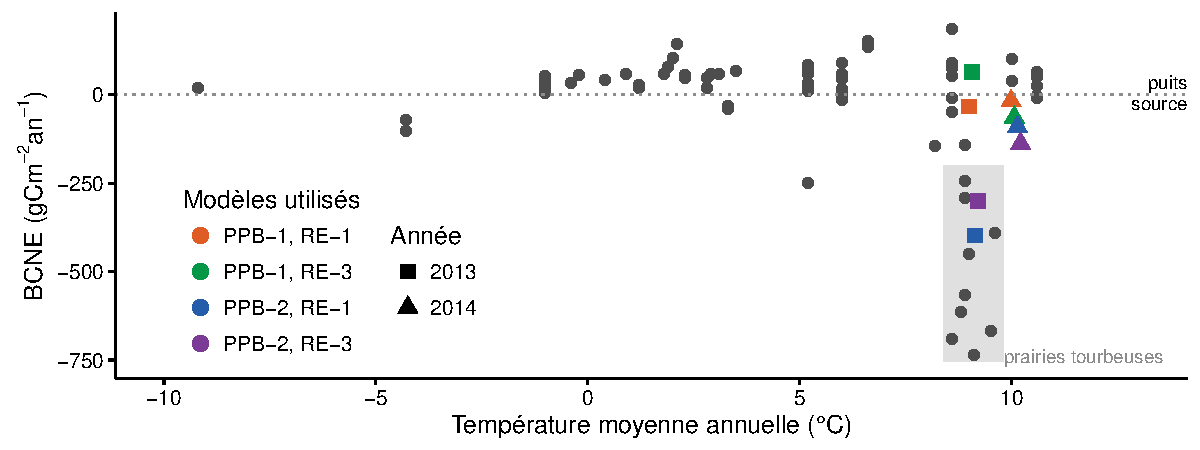
\includegraphics[width=\textwidth]{chap3/bib_vs_necb}
\caption{Relation entre le Bilan de Carbone Net de l'Écosystème (BCNE) et la température moyenne annuelle (en °C) dans la littérature (en gris) et pour ces travaux. La ligne de tirets sépare les écosystèmes stockant du carbone (au dessus) de ceux libérant du carbone (en dessous).}
\label{fig:bib_vs_necb}
\end{figure}


\subsection{Sensibilité et limitations du bilan}

Les incertitudes les plus fortes du bilan sont sur les flux de \chh avec une erreur standard de \SI{32}{\percent} lors de la calibration et de \SI{68}{\percent} lors de la validation.
Cette différence importante montre que l'estimation des flux de \chh à l'aide de l'indice de végétation à permis l'estimation de sa contribution au bilan de carbone de l'écosystème pour les années 2013 et 2014, mais que sont utilisation dans d'autre conditions (année sèche, haute MAT) est fortement limité.
L'importance faible du \chh dans le bilan de carbone de la tourbière rend ces erreurs moins critiques que celles faite sur l'estimation de la PPB.
Les incertitudes importantes sur la PPB, sont mises en évidence par les fortes variations des flux interpolés selon l'équation utilisée.
Elles sont la source des variations observées en termes de bilan.
L'ajout d'un indice de végétation diminue d'incertitude des paramètres du modèle, mais cet apport semble spécifique à l'étude, n'étant pas reflété par l'évaluation dont la végétation est relativement similaire à celle de l'étude spatiale.
À l'inverse la RE est bien contrainte.
Sur les 2 années la différence entre les différentes équations utilisées ne dépassent pas \SI{25}{\gcma}.

\textbf{sensibilité du bilan au variation des paramètres}

\textbf{limitations}
Outre ces aspects ce bilan de carbone est aussi limité par sa représentativité. 
Ainsi la strate arborée fortement présente dans certaines zones n'est pas directement prise en compte.
De la même manière une partie restreinte de la tourbière mais néanmoins présente est constitué de touradons dont l'effet n'a pas été pris en compte.\plop (\textbf{biblio effet microtype}).


\begin{itemize}
\item pas de cartographie (pas grave si p7 maj bien représentée par mdl ecos)
\item extrapolation sur d'autres site difficile (cf validation)
\end{itemize}

\subsection{Représentativité locale du modèle}

Distribution des paramètres

Pourquoi certaines placette mieux que d'autres

Concernant la respiration la représentativité locale des modèles calibrés à l'échelle de l'écosystème semble plus homogène pour le modèle RE-3 que pour le modèle RE-1.

Une telle comparaison entre PPB-1 et PPB-2 n'a pas été possible car vu le faible nombre de données et la qualité relative des modèles PPB par rapport aux modèles RE, peu de modèles sont parvenus à converger pour PPB-1 (11 sur 20 placettes) et pour PPB-2 (17 sur 20 placettes).

\subsection{Bilan de \coo et végétation}

\subsection{Variabilité du recouvrement végétal}

Si quelques placettes proche géographiquement ont des recouvrement végétaux voisins (les placettes p18 et p19 ; p02, p03 et p04 ; p12, p14 et p16) les autres ne présentent pas un tel lien.
Par ailleurs, au sein d'une même classe peuvent être rassemblées des placettes très éloignées spatialement, les placette p01 et p15 par exemple ou les placettes p02 et p17 ou p09 et p20.
Ceci montre une variabilité spatiale importante du recouvrement végétal mais également que cette variabilité ne semble pas zonée géographiquement.

\subsubsection{Effet du type de végétation majoritaire sur les flux de \coo et le bilan de \coo }
Le calcul des bilans avec les différents groupes de végétation permet de mettre en évidence des comportements différents des flux selon la végétation majoritaire.
Ainsi le groupe 3 dans lequel la strate herbacée est la plus importante est celui ou la PPB est la plus forte.
Ce point semble en cohérence avec la croissance annuelle importante des herbacées.
À l'inverse le groupe 1 dans lequel la strate muscinale est la plus importante est également le groupe pour lequel la PPB est la plus faible.
\plop

Pour la RE, ce sont les groupes 3 et 4 qui ont les flux estimés les plus importants avec une différence d'environ \SI{200}{\gcma} avec les deux autres groupes.
Malgré leurs différences, le groupe 2 possède une strate muscinale importante alors qu'elle est absente dans le groupe 3, ils ont en commun d'avoir une strate arbustive importante.


\subsection{perspectives}

cartographie ?

